\documentclass{article} % A4 paper and 11pt font size
\setcounter{secnumdepth}{0}

\usepackage{amssymb, amsmath, amsfonts}
\usepackage{moreverb}
\usepackage{multicol}
\usepackage{graphicx}
\usepackage{enumerate}
\usepackage{caption}
\usepackage{nicefrac}
\usepackage{graphics}
\usepackage[margin=1in]{geometry}
\usepackage{color}
\usepackage{tocloft}
\renewcommand{\cftsecleader}{\cftdotfill{\cftdotsep}}
\usepackage{array}
\usepackage{arydshln}
\usepackage{float}
\usepackage{csquotes}
\usepackage{placeins}
\usepackage{verbatim}
\usepackage{hyperref}
\usepackage{textcomp}
\usepackage[makeroom]{cancel}
\usepackage{bbold}
\usepackage{scrextend}
\usepackage{alltt}
\usepackage{listings}
\usepackage{physics}
\usepackage{mathtools}
\usepackage[normalem]{ulem}
\usepackage{amsthm}
\usepackage{tikz}
\usetikzlibrary{positioning}
\usetikzlibrary{arrows}
\usepackage{pgfplots}
\usepackage{bigints}
\allowdisplaybreaks
\pgfplotsset{compat=1.12}

\theoremstyle{plain}
\newtheorem*{theorem*}{Theorem}
\newtheorem{theorem}{Theorem}
\newtheorem*{lemma*}{Lemma}
\newtheorem{lemma}{Lemma}

\definecolor{verbgray}{gray}{0.9}
% \definecolor{dkgreen}{green}{0.9}

\lstnewenvironment{code}{%
  \lstset{
  language=Python,
  backgroundcolor=\color{verbgray},
  keywordstyle=\color{blue},      % keyword style
  keywordstyle=[2]\color{blue},   % keyword style
  commentstyle=\color{magenta},   % comment style
  stringstyle=\color{olive},      % string literal styleframe=single,
  numberstyle=\color{black},      % string literal styleframe=single,
  framerule=0pt,
  numbers=left,
  stepnumber=1,
  firstnumber=1,
  showspaces=false,
  basicstyle=\ttfamily}}{}

\lstnewenvironment{console_output}{%
  \lstset{
  framerule=0pt,
  numbers=left,
  stepnumber=1,
  showspaces=false,
  firstnumber=1,
  basicstyle=\ttfamily}}{}


\makeatletter
\newcommand{\BIGG}{\bBigg@{3}}
\newcommand{\vast}{\bBigg@{4}}
\newcommand{\Vast}{\bBigg@{5}}
\makeatother

\newenvironment{definition}[1][Definition]{\begin{trivlist}
\item[\hskip \labelsep {\bfseries #1}]}{\end{trivlist}}

\newcommand{\dy}{\partial_y}
\newcommand{\dyy}{\partial_{yy}}
\newcommand{\dxx}{\partial_{xx}}
\newcommand{\dxy}{\partial_{xy}}
\newcommand{\dyyy}{\partial_{yyy}}
\newcommand{\dxxx}{\partial_{xxx}}
\newcommand{\dx}{\partial_x}
\newcommand{\E}{\varepsilon}
\def\Rl{\mathbb{R}}
\def\Cx{\mathbb{C}}

\newcommand{\Ei}{\text{Ei}}

\usepackage[T1]{fontenc} % Use 8-bit encoding that has 256 glyphs
\usepackage{fourier} % Use the Adobe Utopia font for the document - comment this line to return to the LaTeX default
\usepackage[english]{babel} % English language/hyphenation

\usepackage{sectsty} % Allows customizing section commands
\allsectionsfont{\centering \normalfont\scshape} % Make all sections centered, the default font and small caps

\usepackage{fancyhdr} % Custom headers and footers
\pagestyle{fancy} % Makes all pages in the document conform to the custom headers and footers
\fancyhead[L]{\bf Sam Fleischer}
\fancyhead[C]{\bf UC Davis \\ Numerical Solutions of Differential Equations (MAT228A)} % No page header - if you want one, create it in the same way as the footers below
\fancyhead[R]{\bf Fall 2016}

\fancyfoot[L]{\bf } % Empty left footer
\fancyfoot[C]{\bf \thepage} % Empty center footer
\fancyfoot[R]{\bf } % Page numbering for right footer
\renewcommand{\headrulewidth}{0pt} % Remove header underlines
\renewcommand{\footrulewidth}{0pt} % Remove footer underlines
\setlength{\headheight}{25pt} % Customize the height of the header

\newcommand{\VEC}[2]{\left\langle #1, #2 \right\rangle}
\newcommand{\ran}{\text{\rm ran }}
\newcommand{\Hilb}{\mathcal{H}}
\newcommand{\lap}{\Delta}

\newcommand{\littleo}[1]{\text{\scriptsize$\mathcal{O}$}\qty(#1)}

\DeclareMathOperator*{\esssup}{\text{ess~sup}}

\newcommand{\problem}[2]{
\vspace{.375cm}
\boxed{\begin{minipage}{\textwidth}
    \section{\bf #1}
    #2
\end{minipage}}
}

\numberwithin{equation}{section} % Number equations within sections (i.e. 1.1, 1.2, 2.1, 2.2 instead of 1, 2, 3, 4)
\numberwithin{figure}{section} % Number figures within sections (i.e. 1.1, 1.2, 2.1, 2.2 instead of 1, 2, 3, 4)
\numberwithin{table}{section} % Number tables within sections (i.e. 1.1, 1.2, 2.1, 2.2 instead of 1, 2, 3, 4)

\setlength\parindent{0pt} % Removes all indentation from paragraphs - comment this line for an assignment with lots of text

\newcommand{\horrule}[1]{\rule{\linewidth}{#1}} % Create horizontal rule command with 1 argument of height

\title{ 
\normalfont \normalsize 
\textsc{UC Davis, Numerical Solutions of Differential Equations (MAT 228A), Fall 2016} \\ [25pt] % Your university, school and/or department name(s)
\horrule{2pt} \\[0.4cm] % Thin top horizontal rule
\Huge Homework \#3 \\ % The assignment title
\horrule{2pt} \\[0.5cm] % Thick bottom horizontal rule
}

\author{\huge Sam Fleischer} % Your name

\date{November 11, 2016} % Today's date or a custom date

\begin{document}\thispagestyle{empty}

\maketitle % Print the title

\makeatletter
\@starttoc{toc}
\makeatother

\pagebreak

%%%%%%%%%%%%%%%%%%%%%%%%%%%%%%%%%%%%%%
\problem{Problem 1}{Use Jacobi, Gauss-Seidel, and SOR (with optimal $\omega$) to solve
\begin{align*}
    \laplacian u = -\exp(-(x - 0.25)^2 - (y - 0.6)^2)
\end{align*}
on the unit square $(0,1)\times(0,1)$ with homogeneous Dirichlet boundary conditions.  Find the solution for mesh spacings of $h = 2^{-5}$, $2^{-6}$, and $2^{-7}$.  What tolerance did you use?  What stopping criteria did you use?  What value of $\omega$ did you use?  Report the number of iterations it took to reach convergence for each method for each mesh.
}

I used the following iterative methods to solve
\begin{align*}
    \laplacian u = -\exp(-(x - 0.25)^2 - (y - 0.6)^2)
\end{align*}
on the unit square with grid size $2^{-i}$ for $i = 5,6,7$:
\begin{itemize}
    \item Jacobi:
    \begin{align*}
        u_{i,j}^{k+1} = \frac{1}{4}\qty(u_{i-1,j}^k + u_{i+1,j}^k + u_{i,j-1}^k + u_{i,j+1}^k - h^2f_{i,j})
    \end{align*}
    Here are the results for $h = 2^{-i}$ for $i=5,6,7$.
    \begin{figure}[ht!]
        \centering
        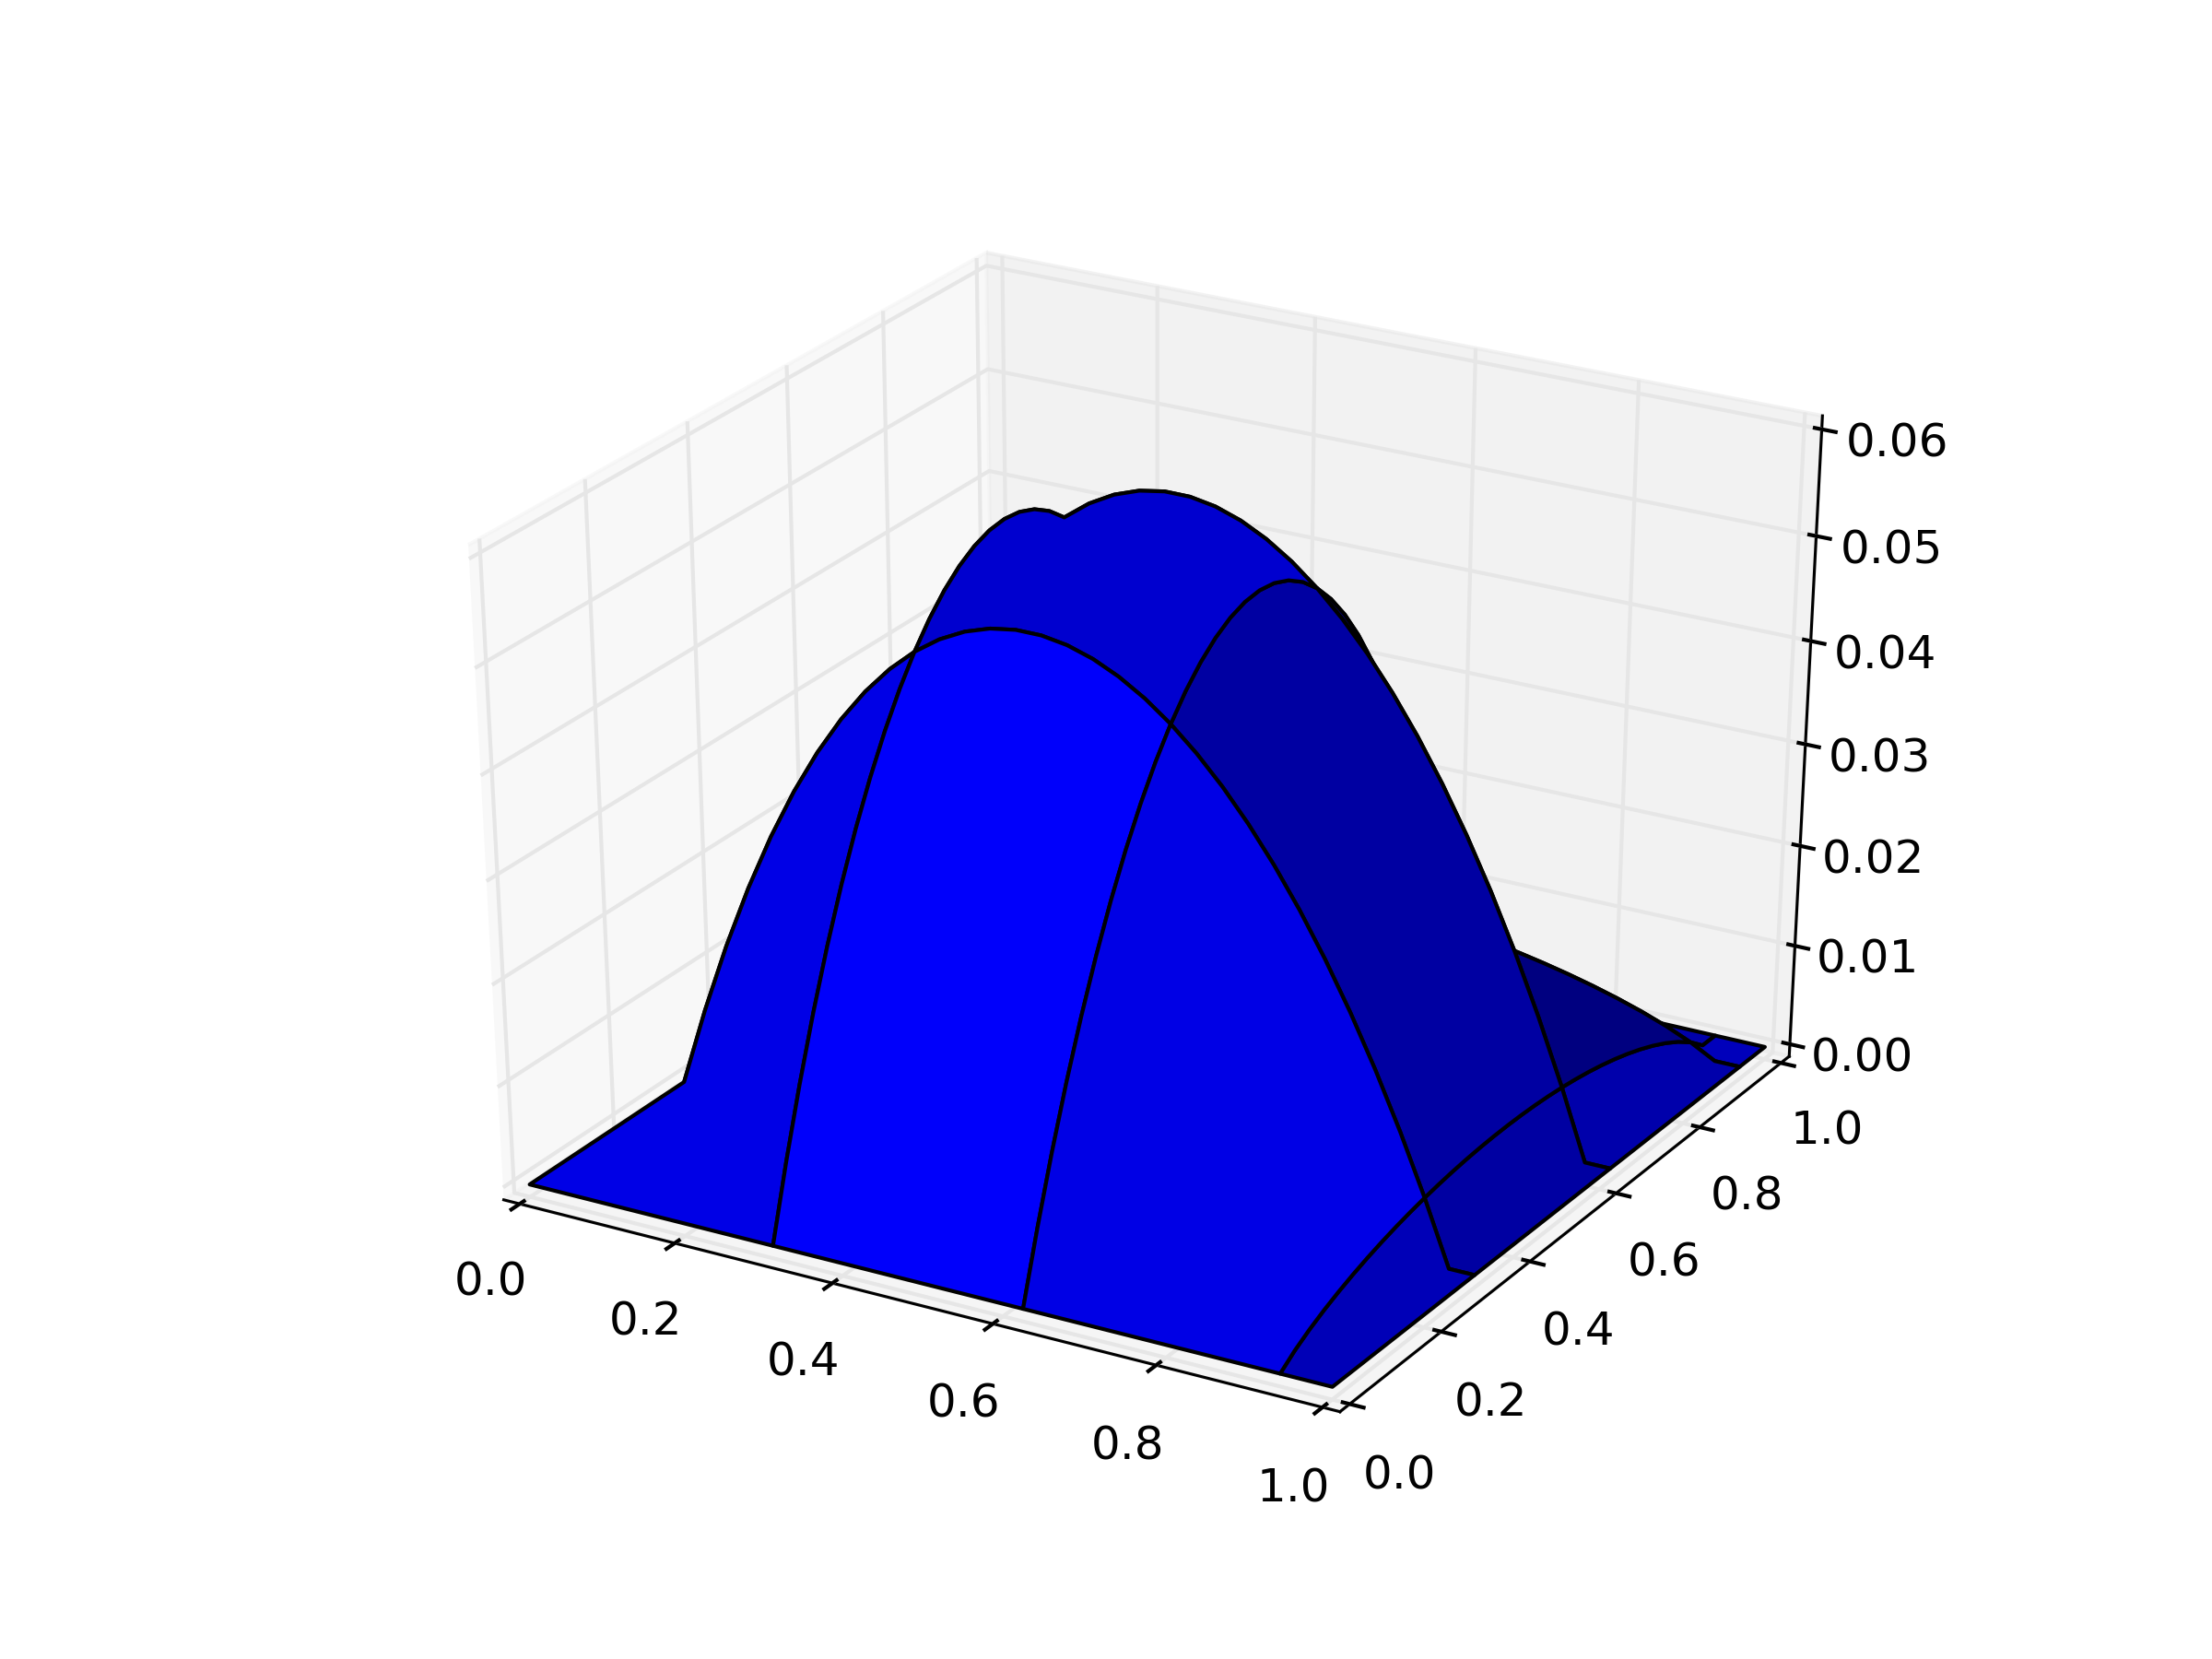
\includegraphics[width=0.3\textwidth]{figure_1_jacobi_0.png}
        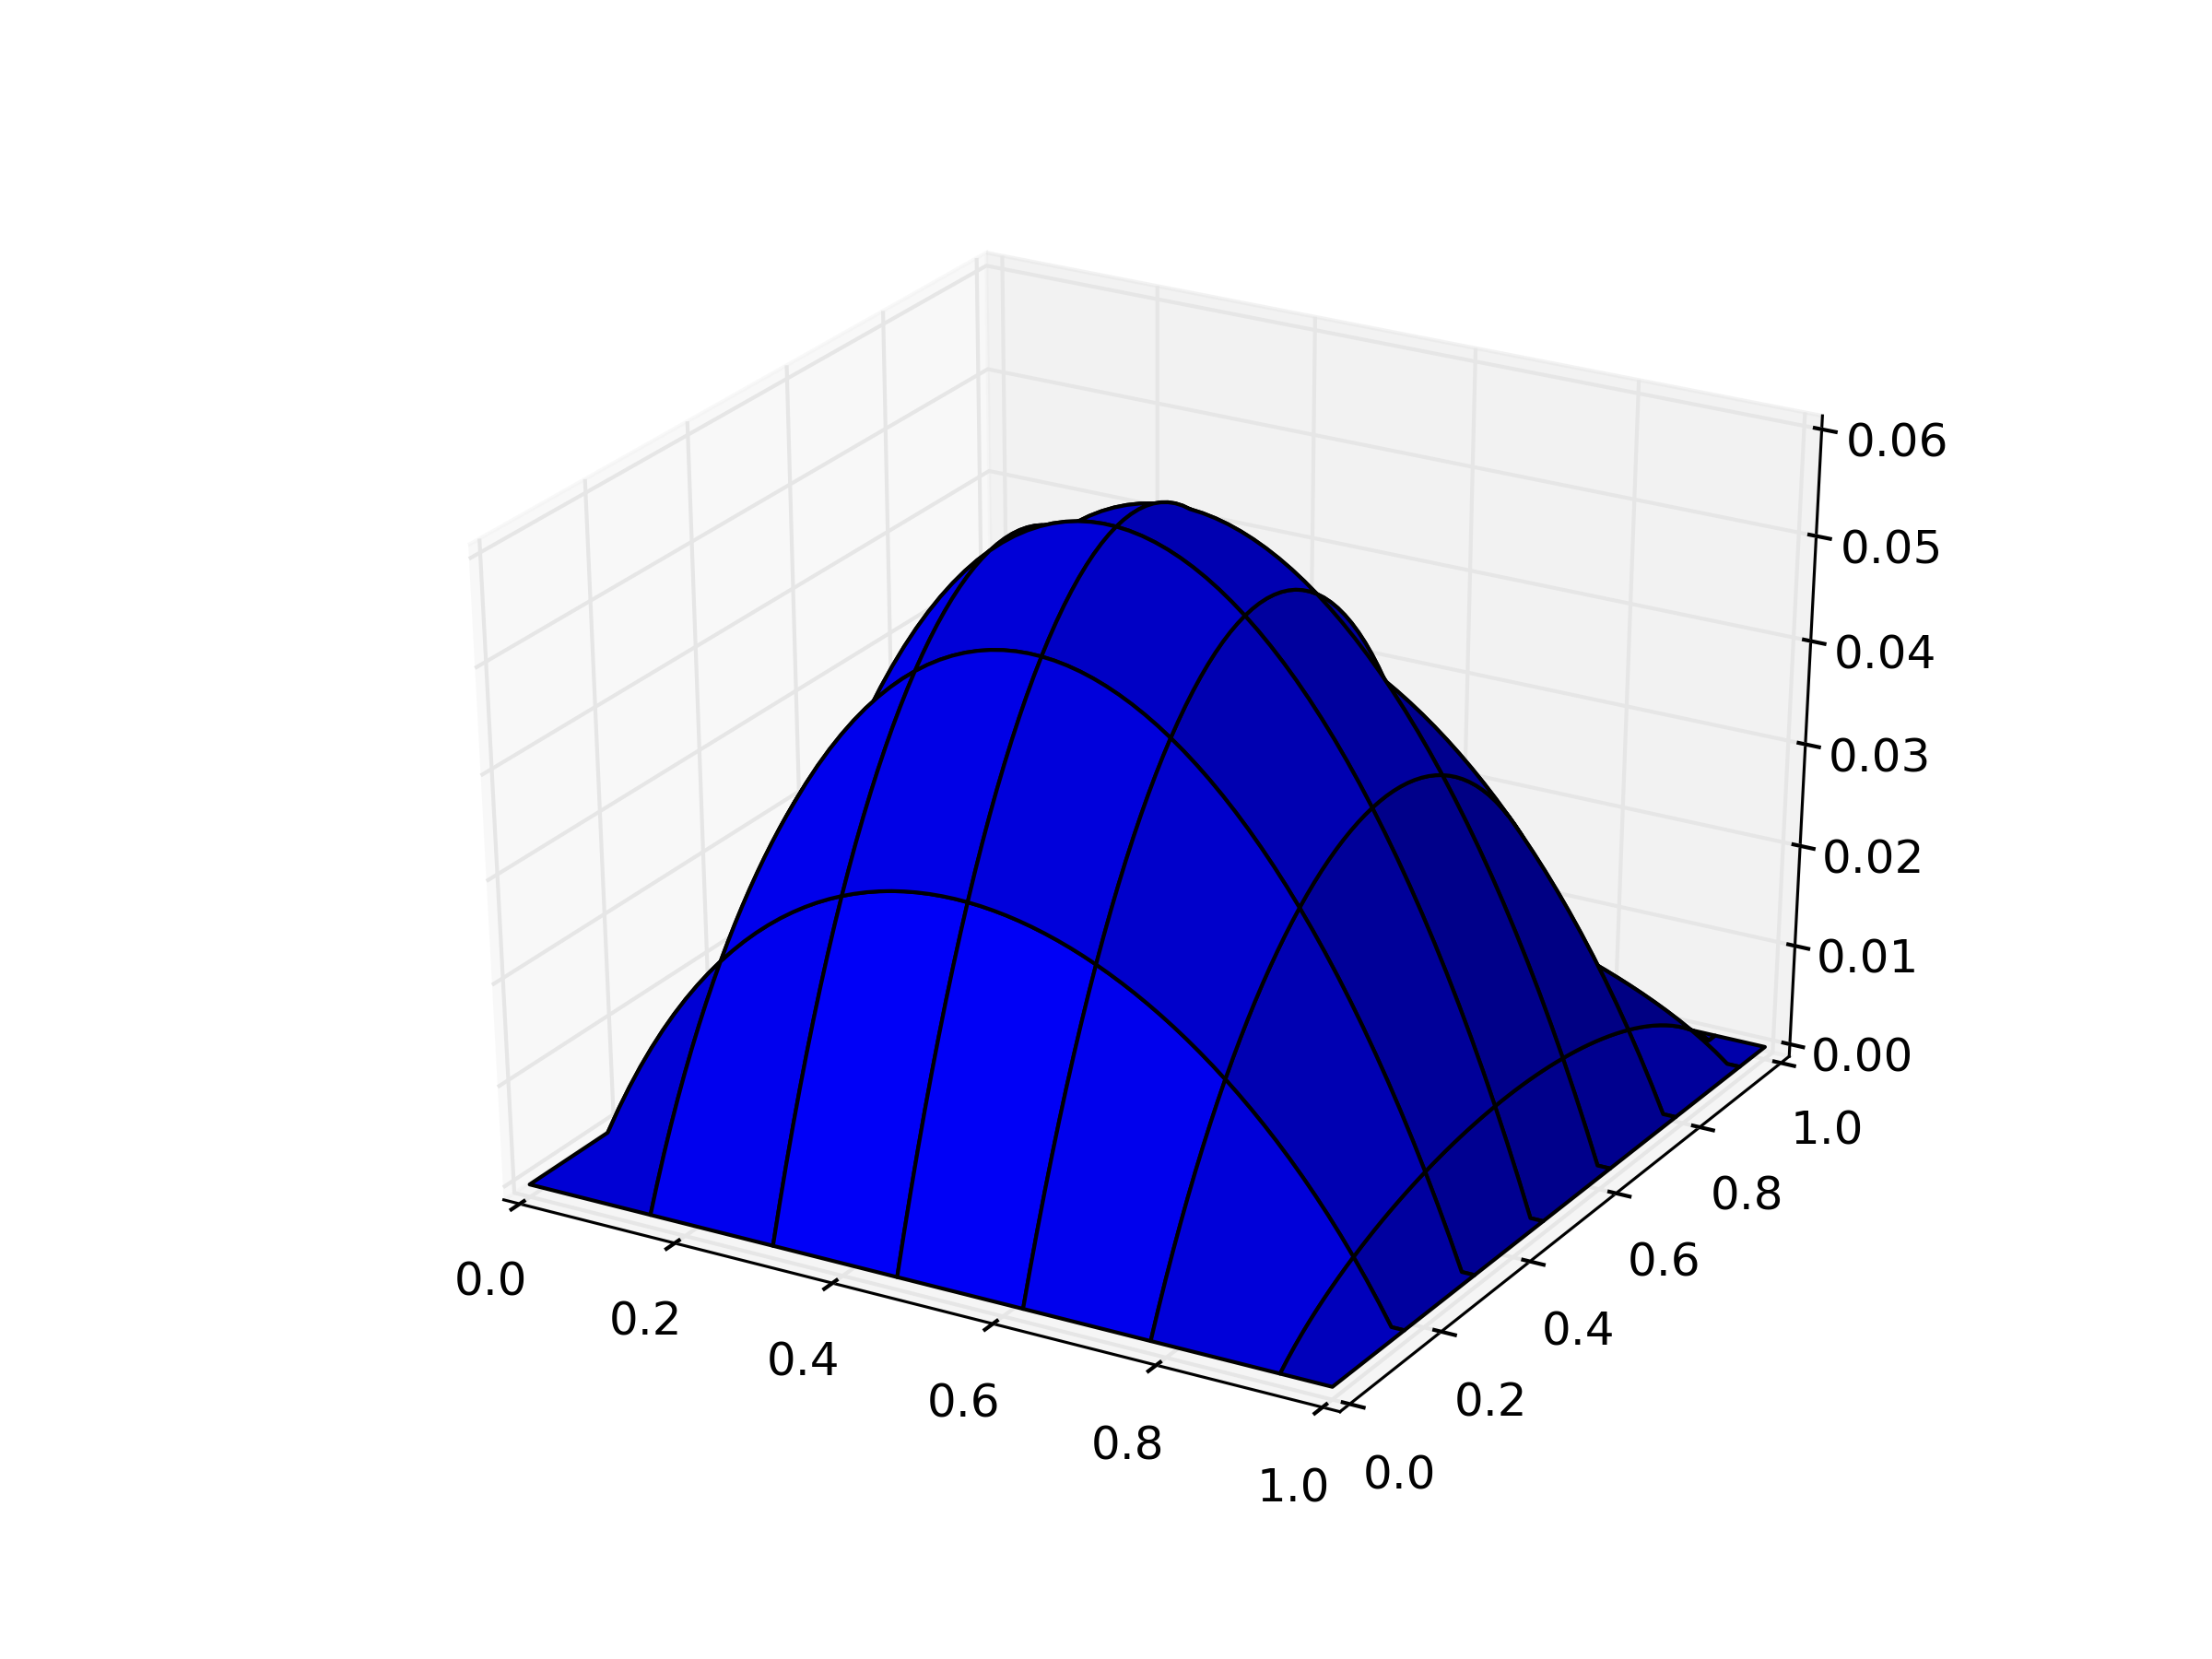
\includegraphics[width=0.3\textwidth]{figure_1_jacobi_1.png}
        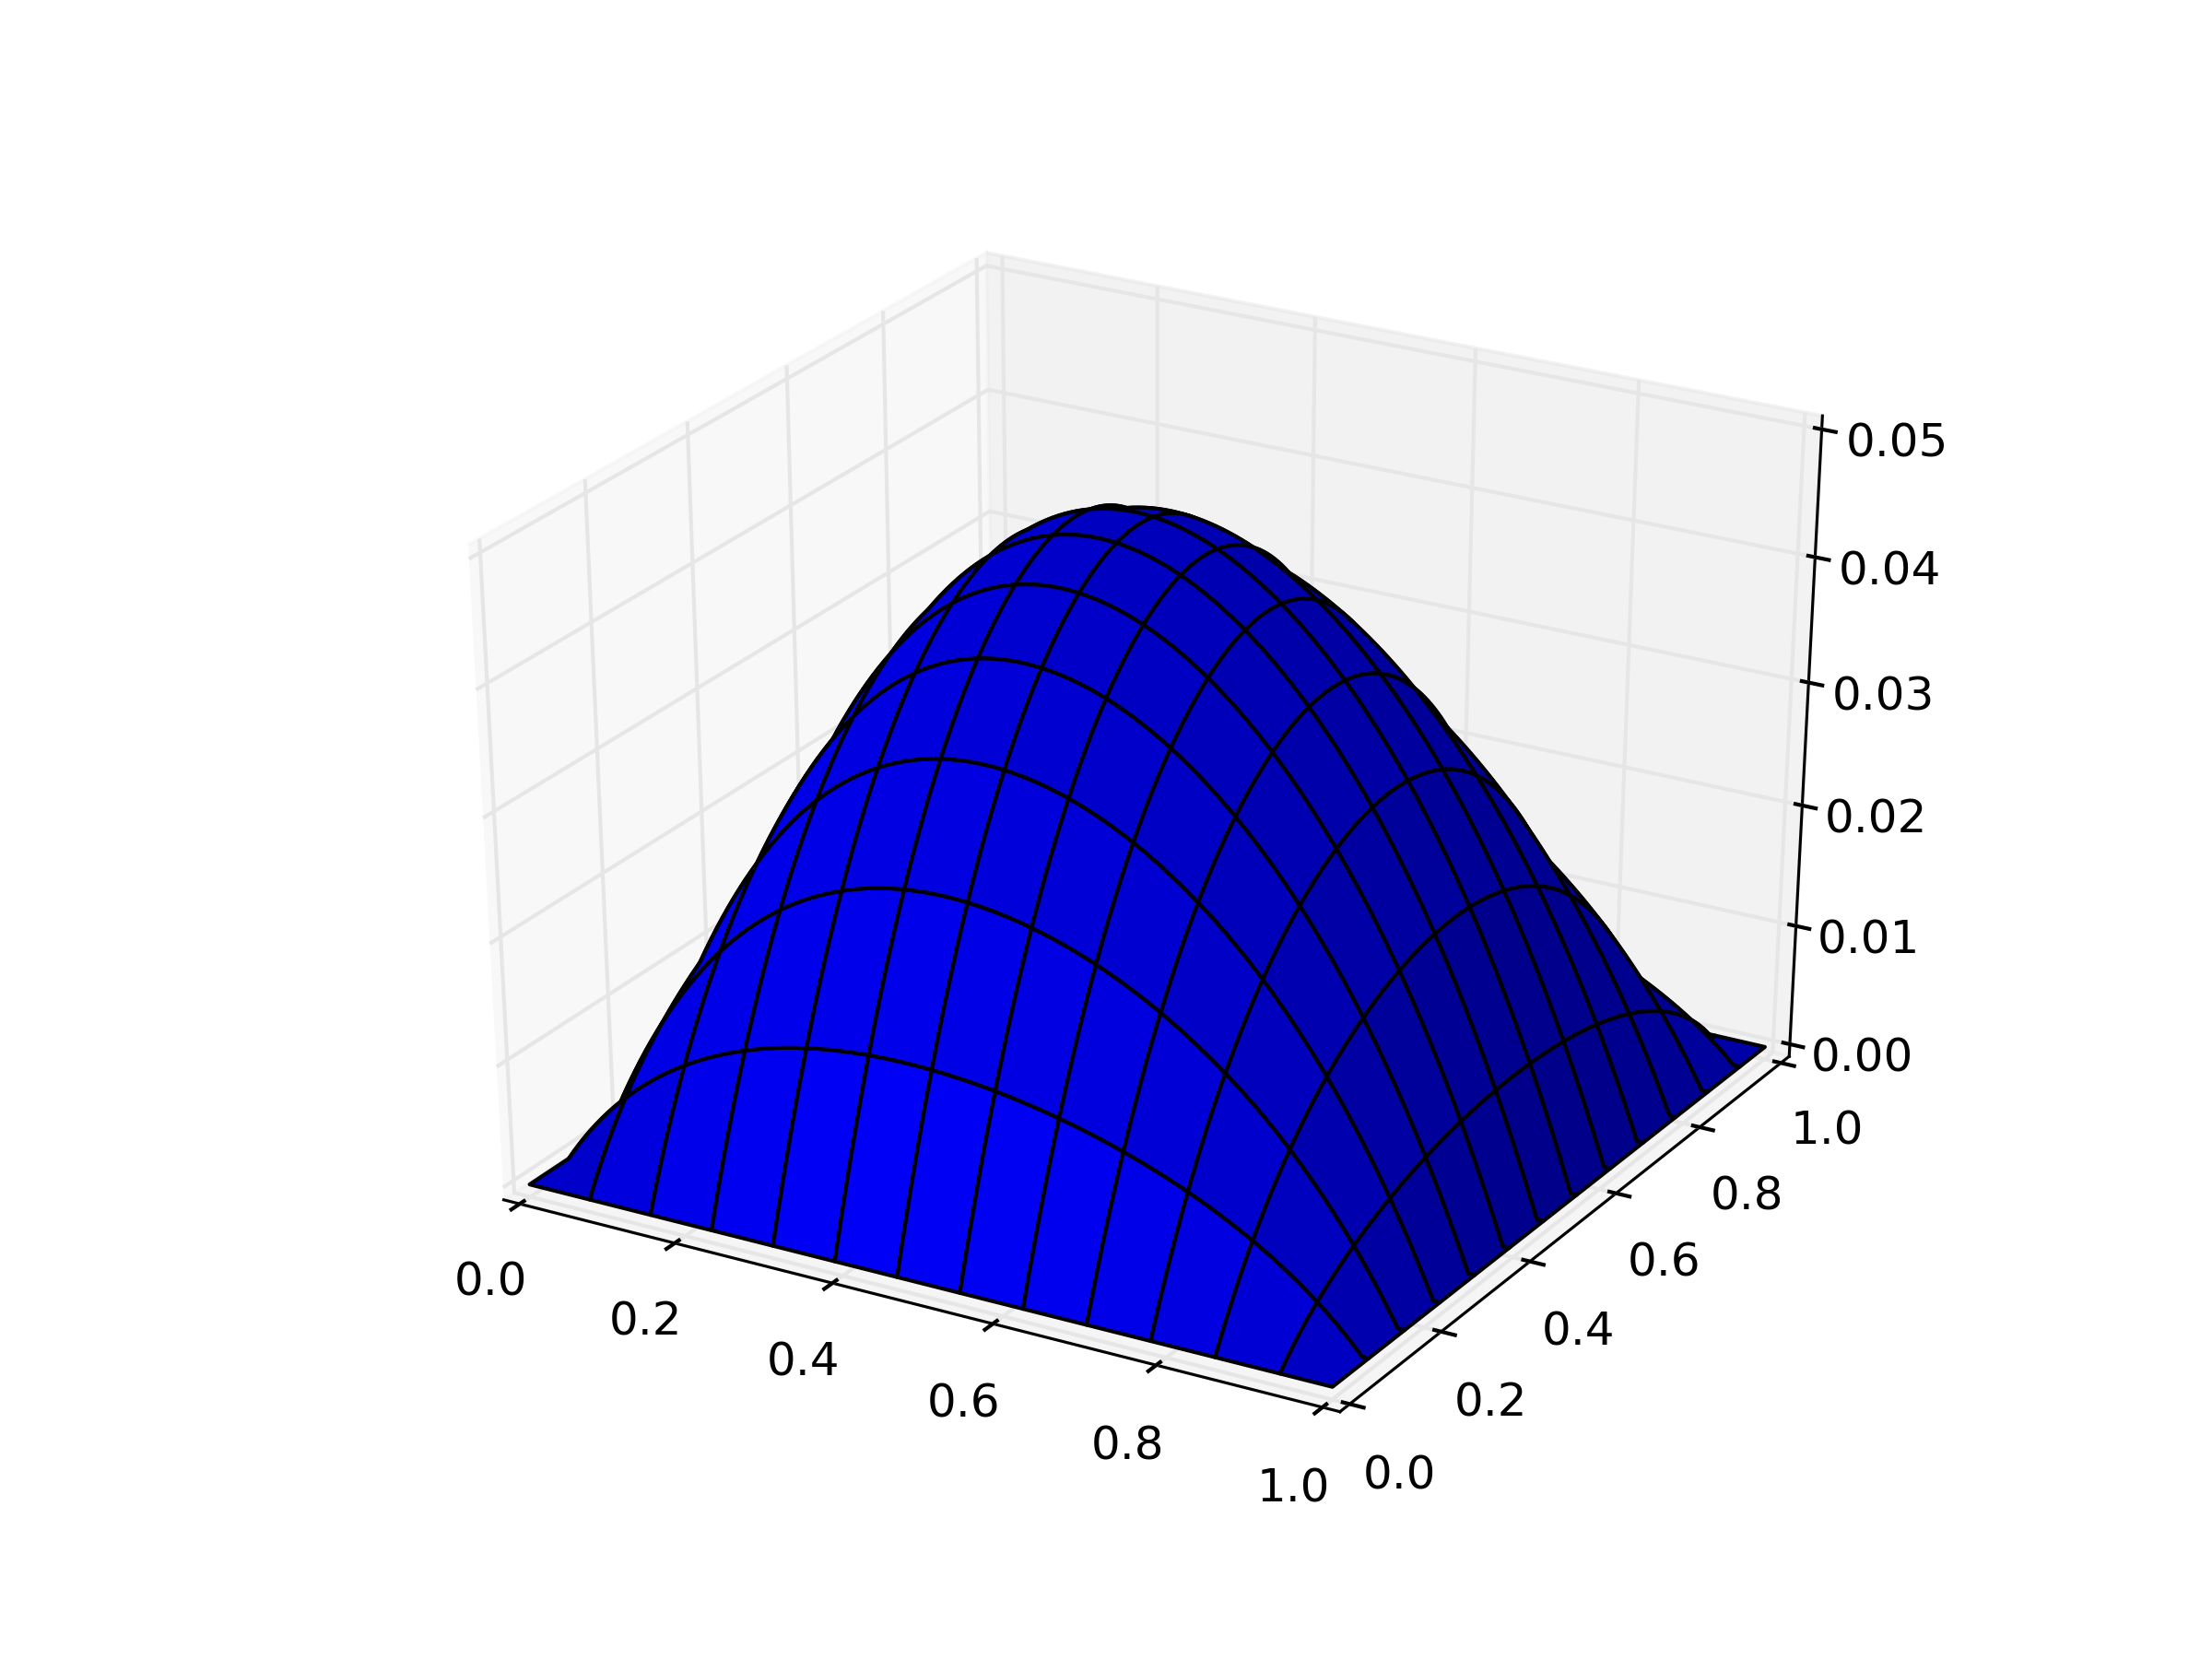
\includegraphics[width=0.3\textwidth]{figure_1_jacobi_2.png}
    \end{figure}
    \FloatBarrier
    The number of iterations required to have a relative error less than $0.0001$ (that is, $\norm{u^{k+1} - u^k}_1 < \E\norm{u_k}_1$, where $\E = 0.0001$) is
    \begin{align*}
        \begin{array}{||l|l|l|l||}\hline\hline
            h & \text{iterations} & \text{multiplicative factor} & \text{time taken (in seconds)} \\[.1cm]\hline\hline
            2^{-5} & 1377 & & 3.549528 \\[.1cm]\hline
            2^{-6} & 4570 & 3.32 & 44.084062 \\[.1cm]\hline
            2^{-7} & 14607 & 3.20 & 575.336392\\[.1cm]\hline\hline
        \end{array}
    \end{align*}
    Here is a graph of the relative errors as a function of the iteration number:
    \begin{figure}[ht!]
        \centering
        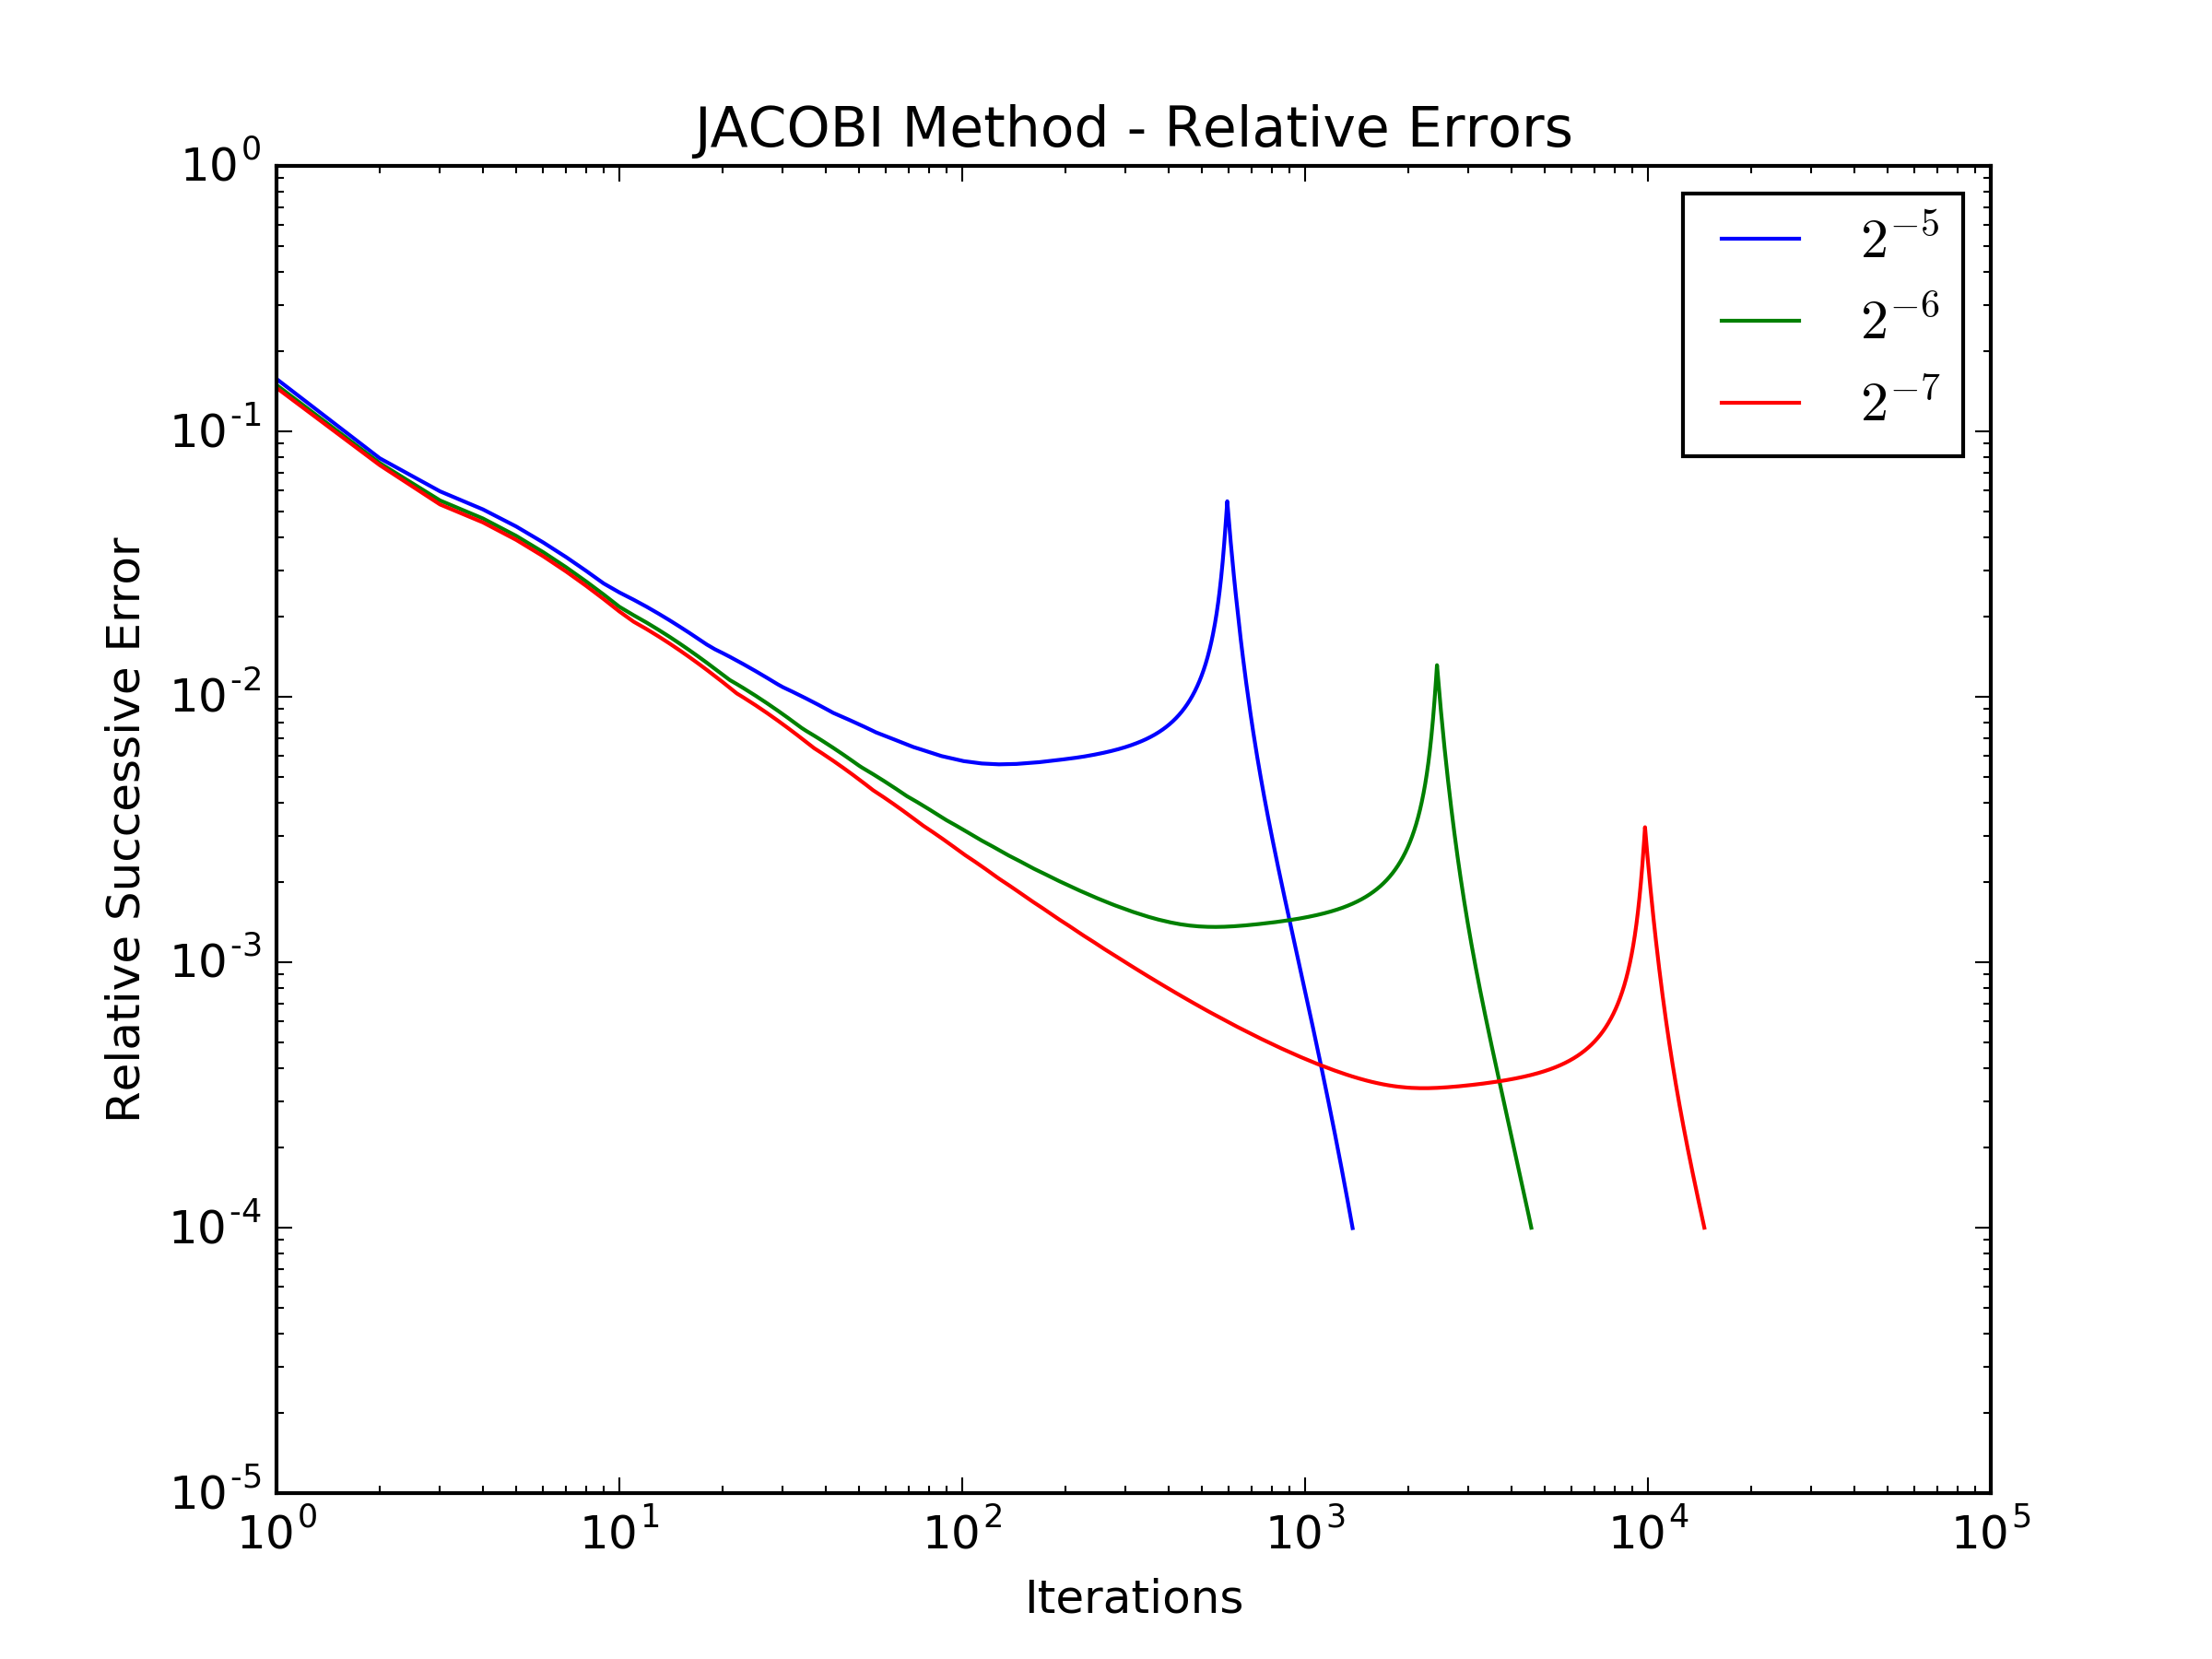
\includegraphics[width=0.5\textwidth]{figure_1_error_jacobi.png}
    \end{figure}
    \FloatBarrier
    \item Gauss-Seidel
    \begin{align*}
        u_{i,j}^{k+1} = \frac{1}{4}\qty(u_{i-1,j}^{k+1} + u_{i+1,j}^k + u_{i,j-1}^{k+1} + u_{i,j+1}^k - h^2f_{i,j})
    \end{align*}
    Here are the results for $h = 2^{-i}$ for $i=5,6,7$.
    \begin{figure}[ht!]
        \centering
        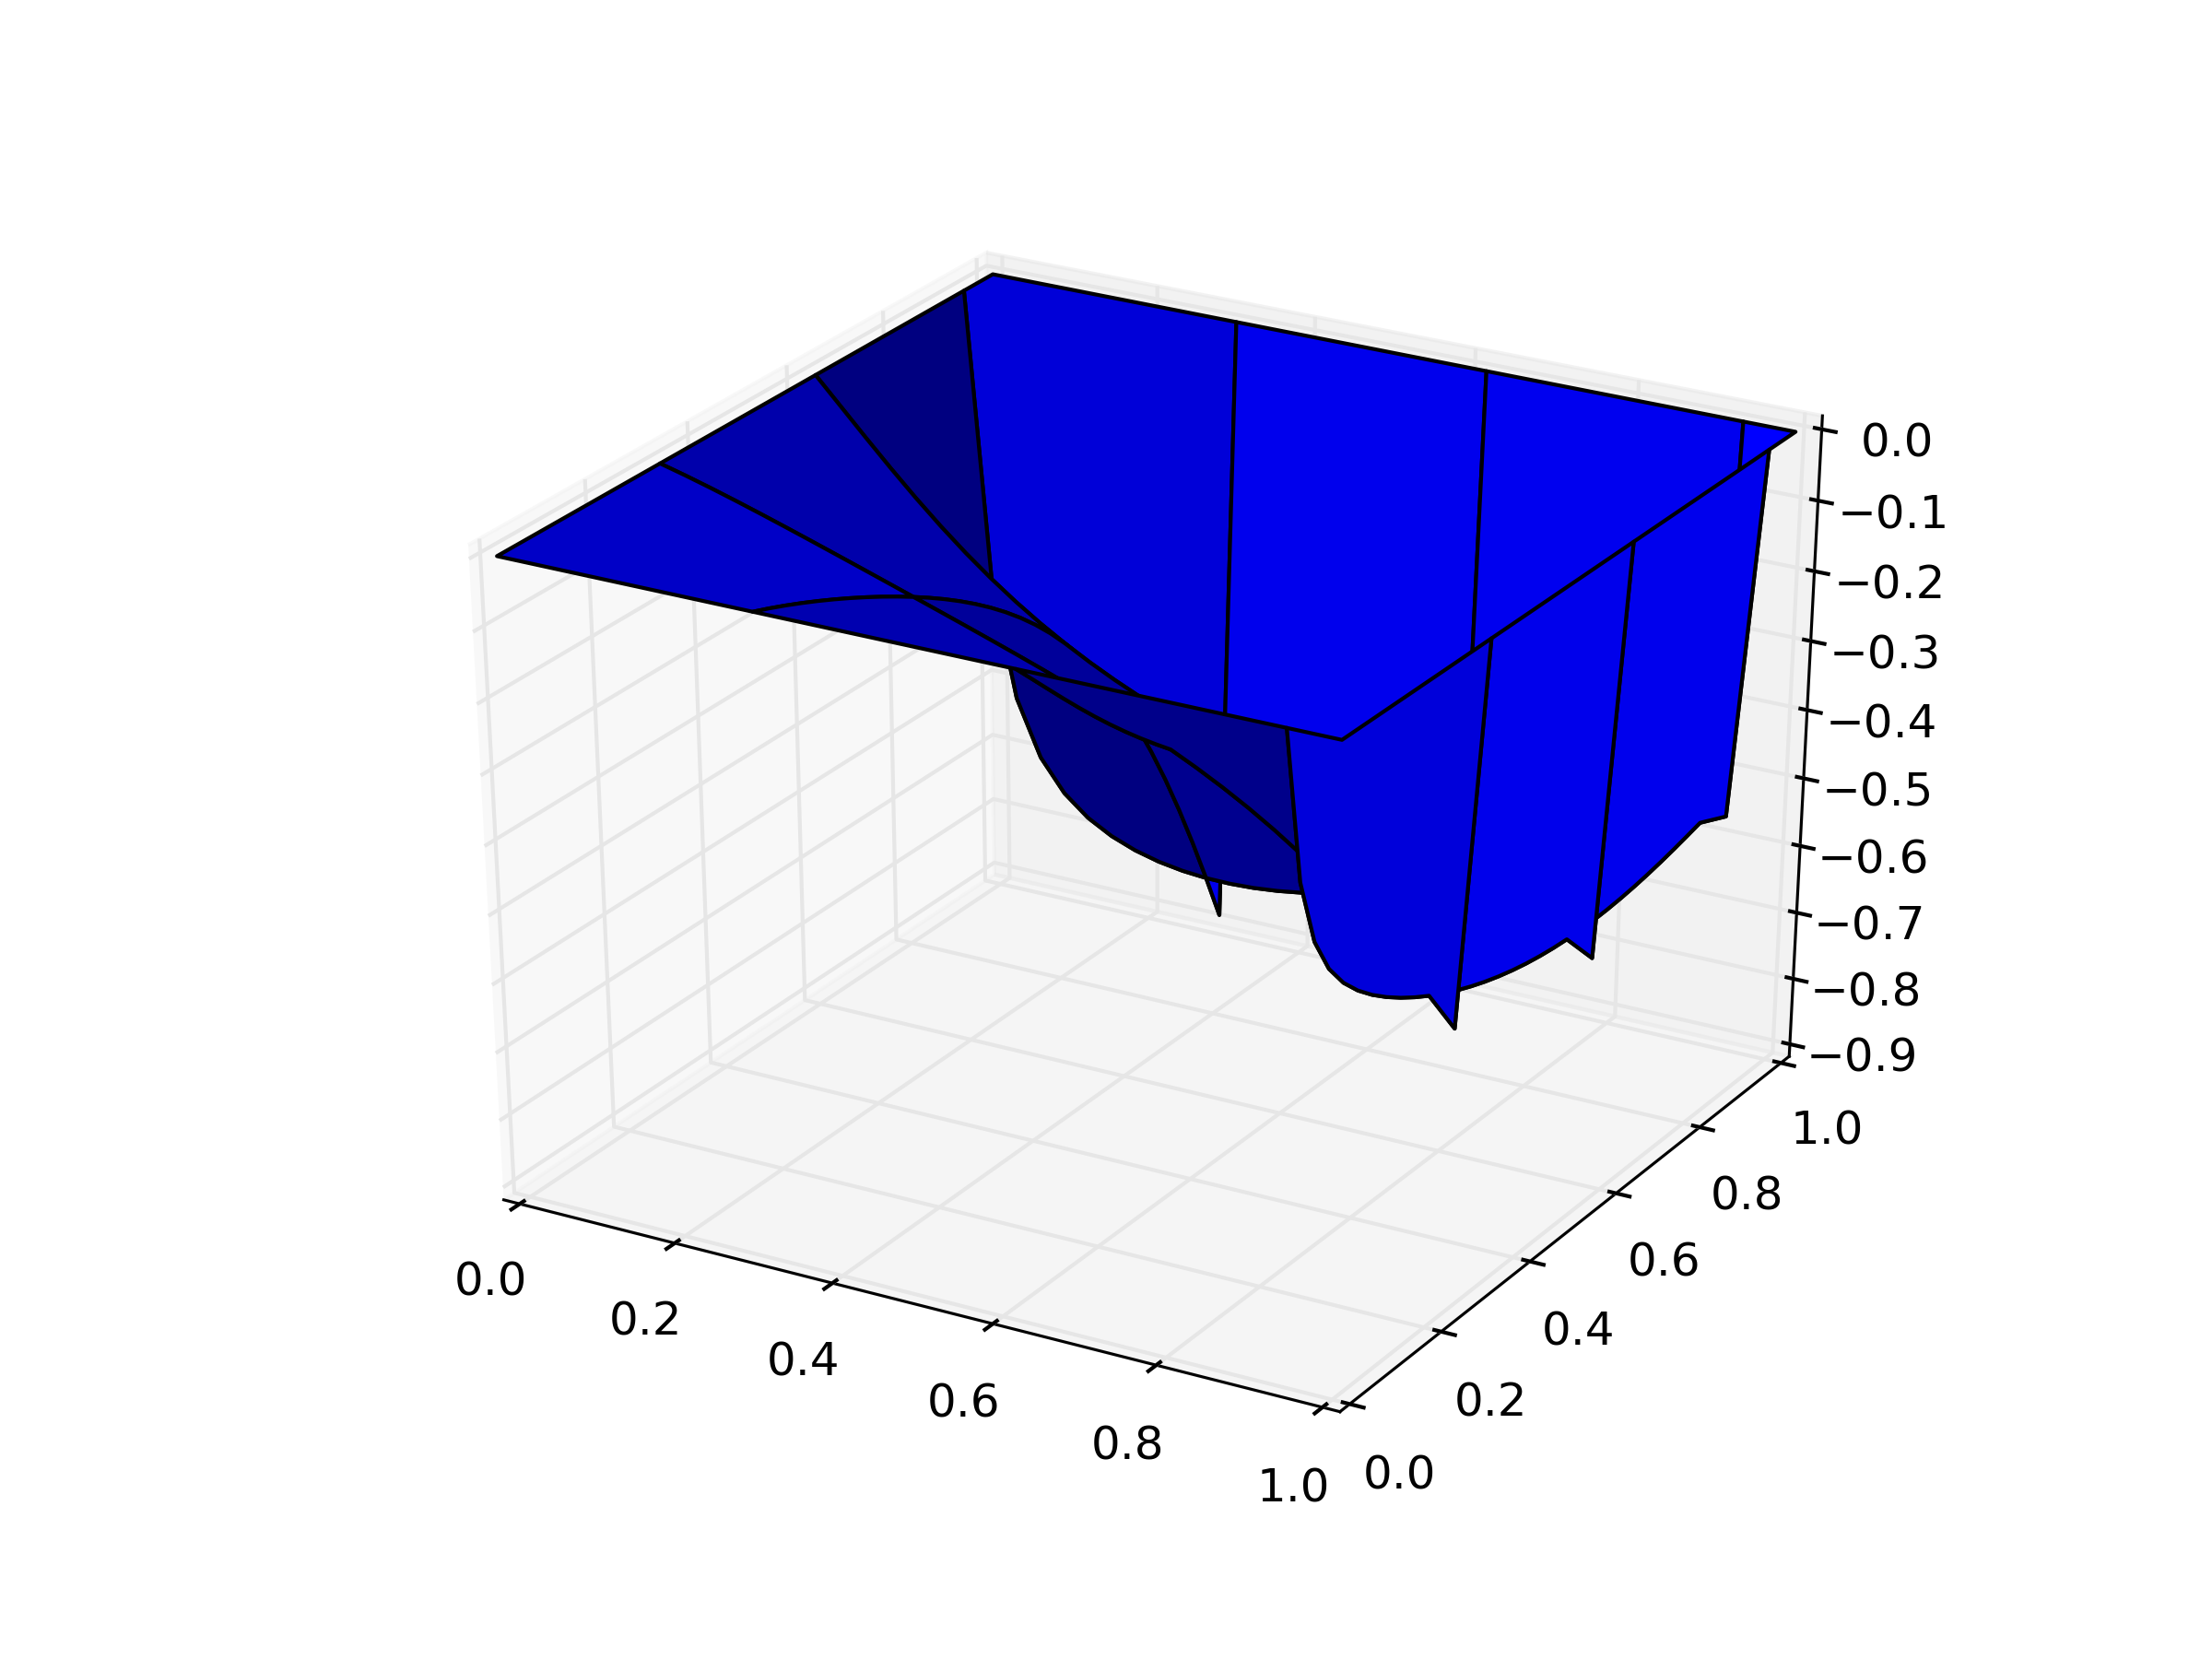
\includegraphics[width=0.3\textwidth]{figure_1_gs_0.png}
        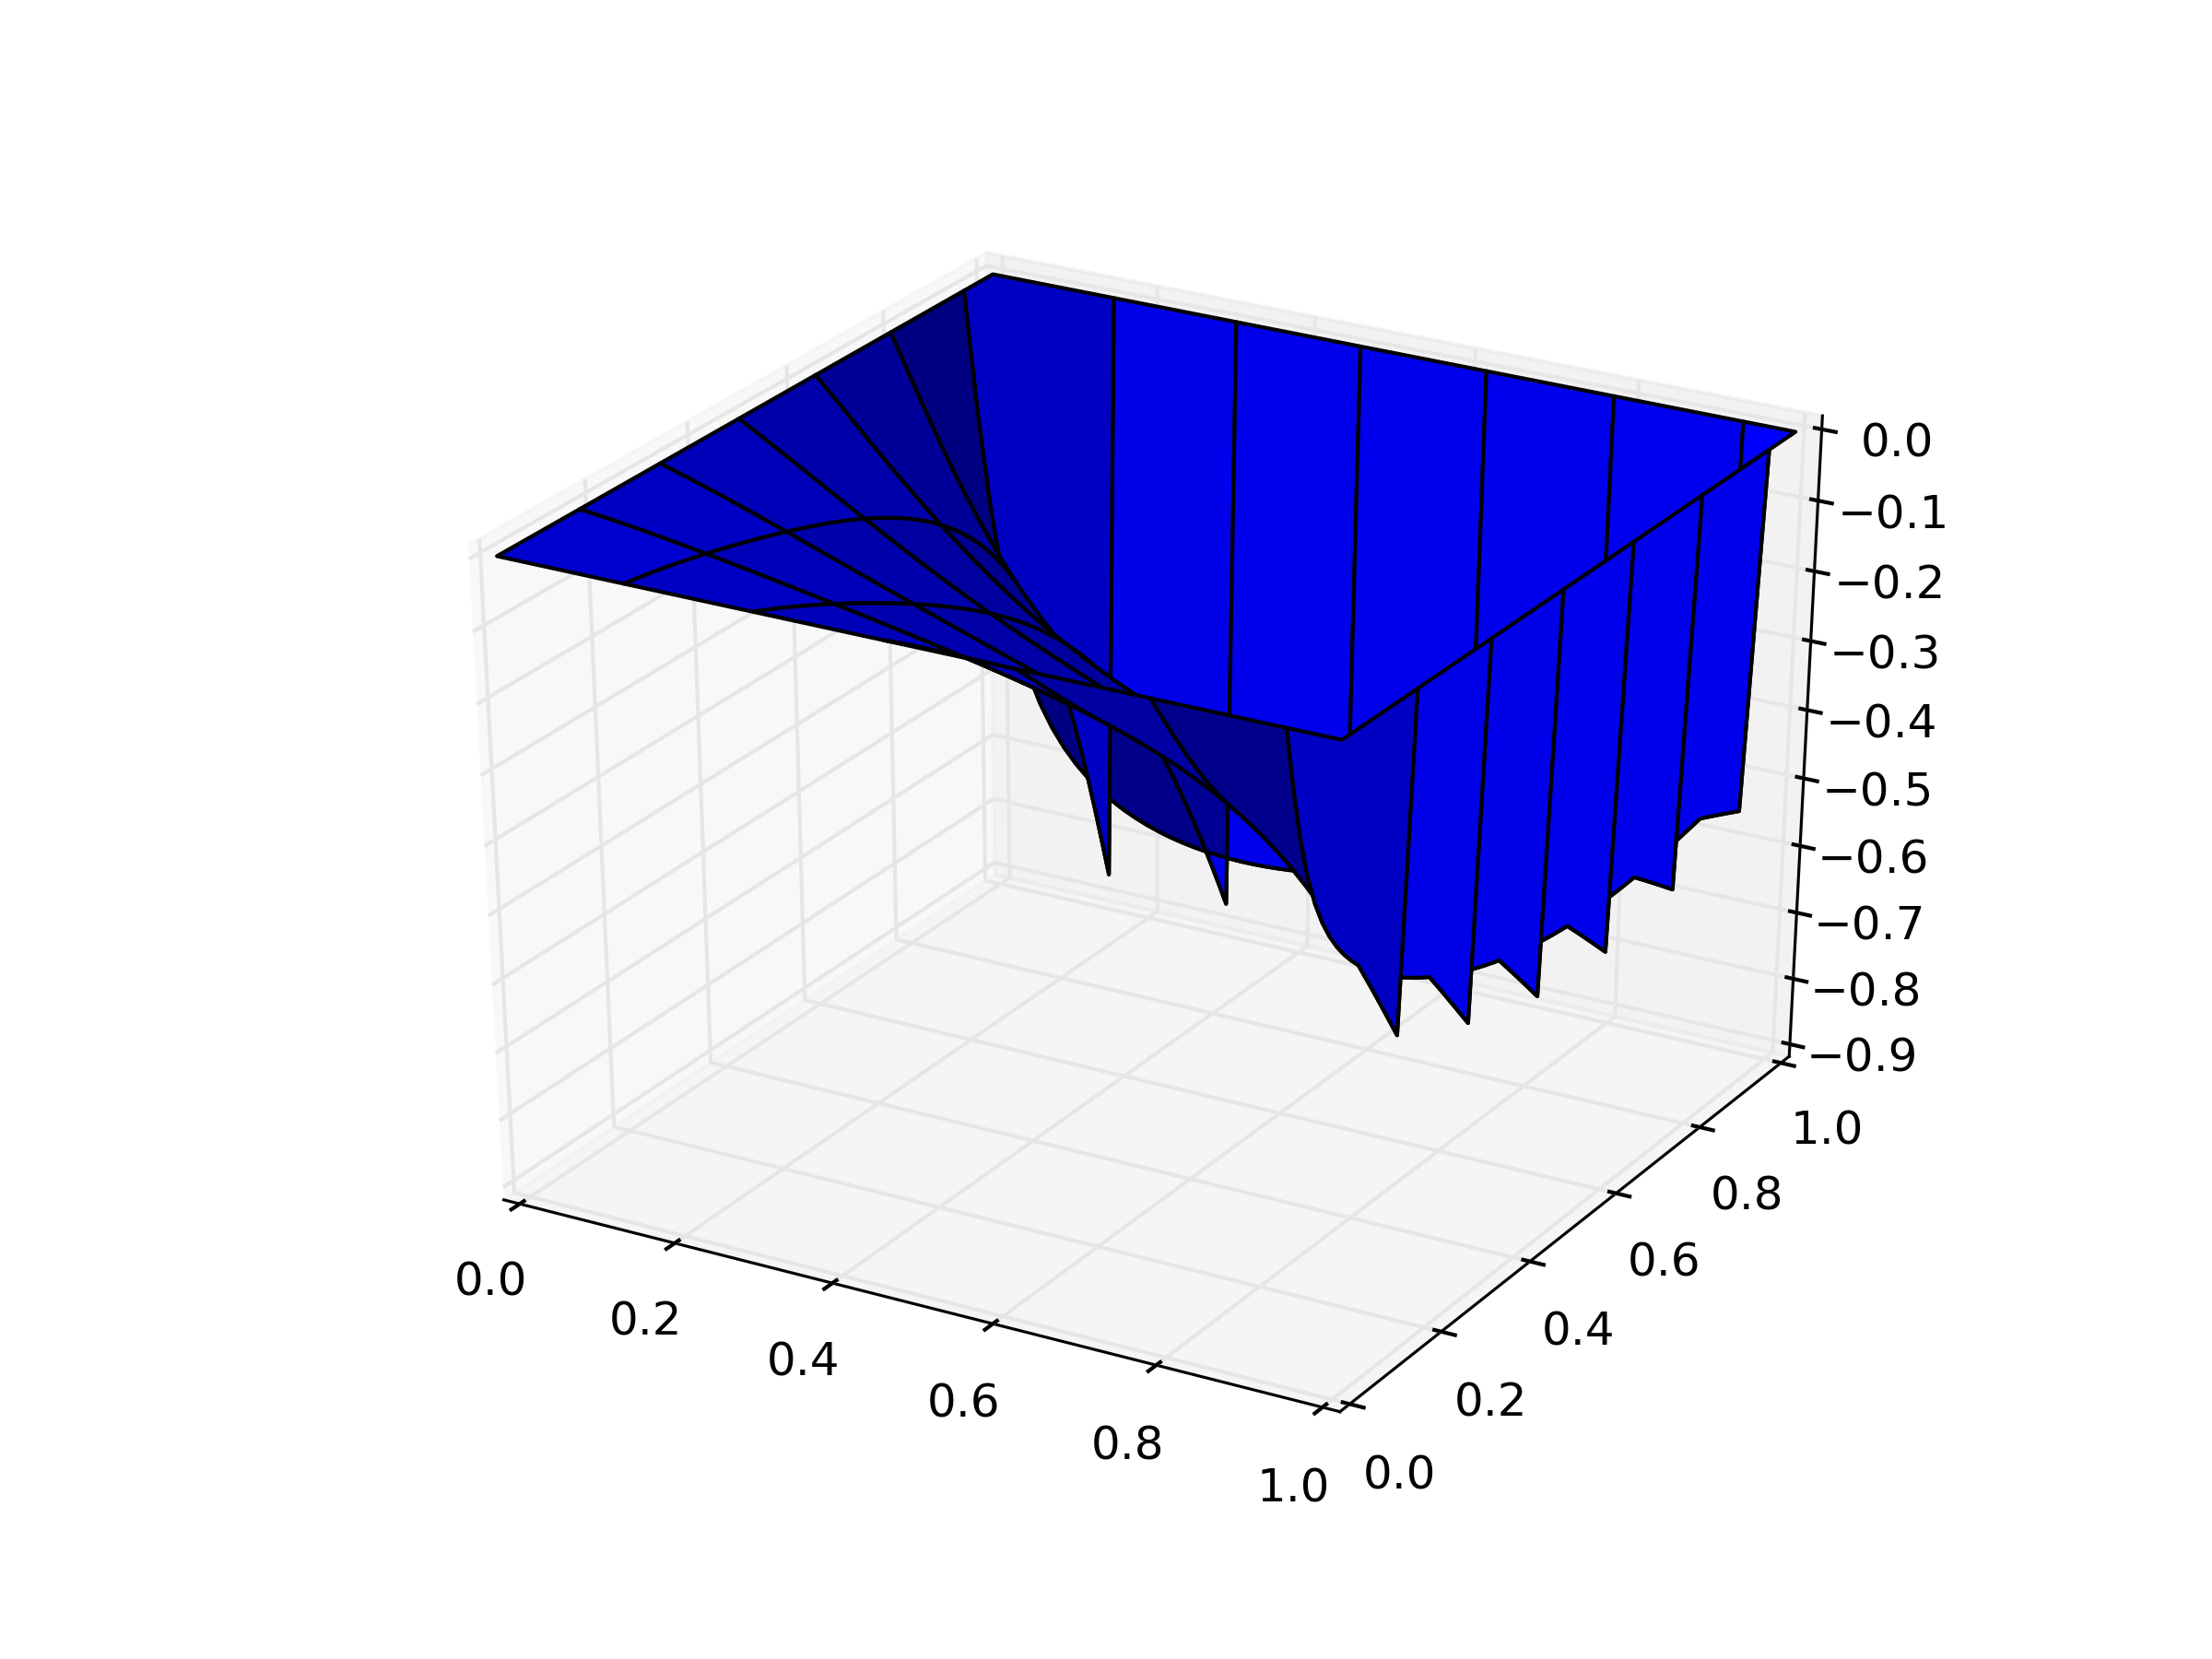
\includegraphics[width=0.3\textwidth]{figure_1_gs_1.png}
        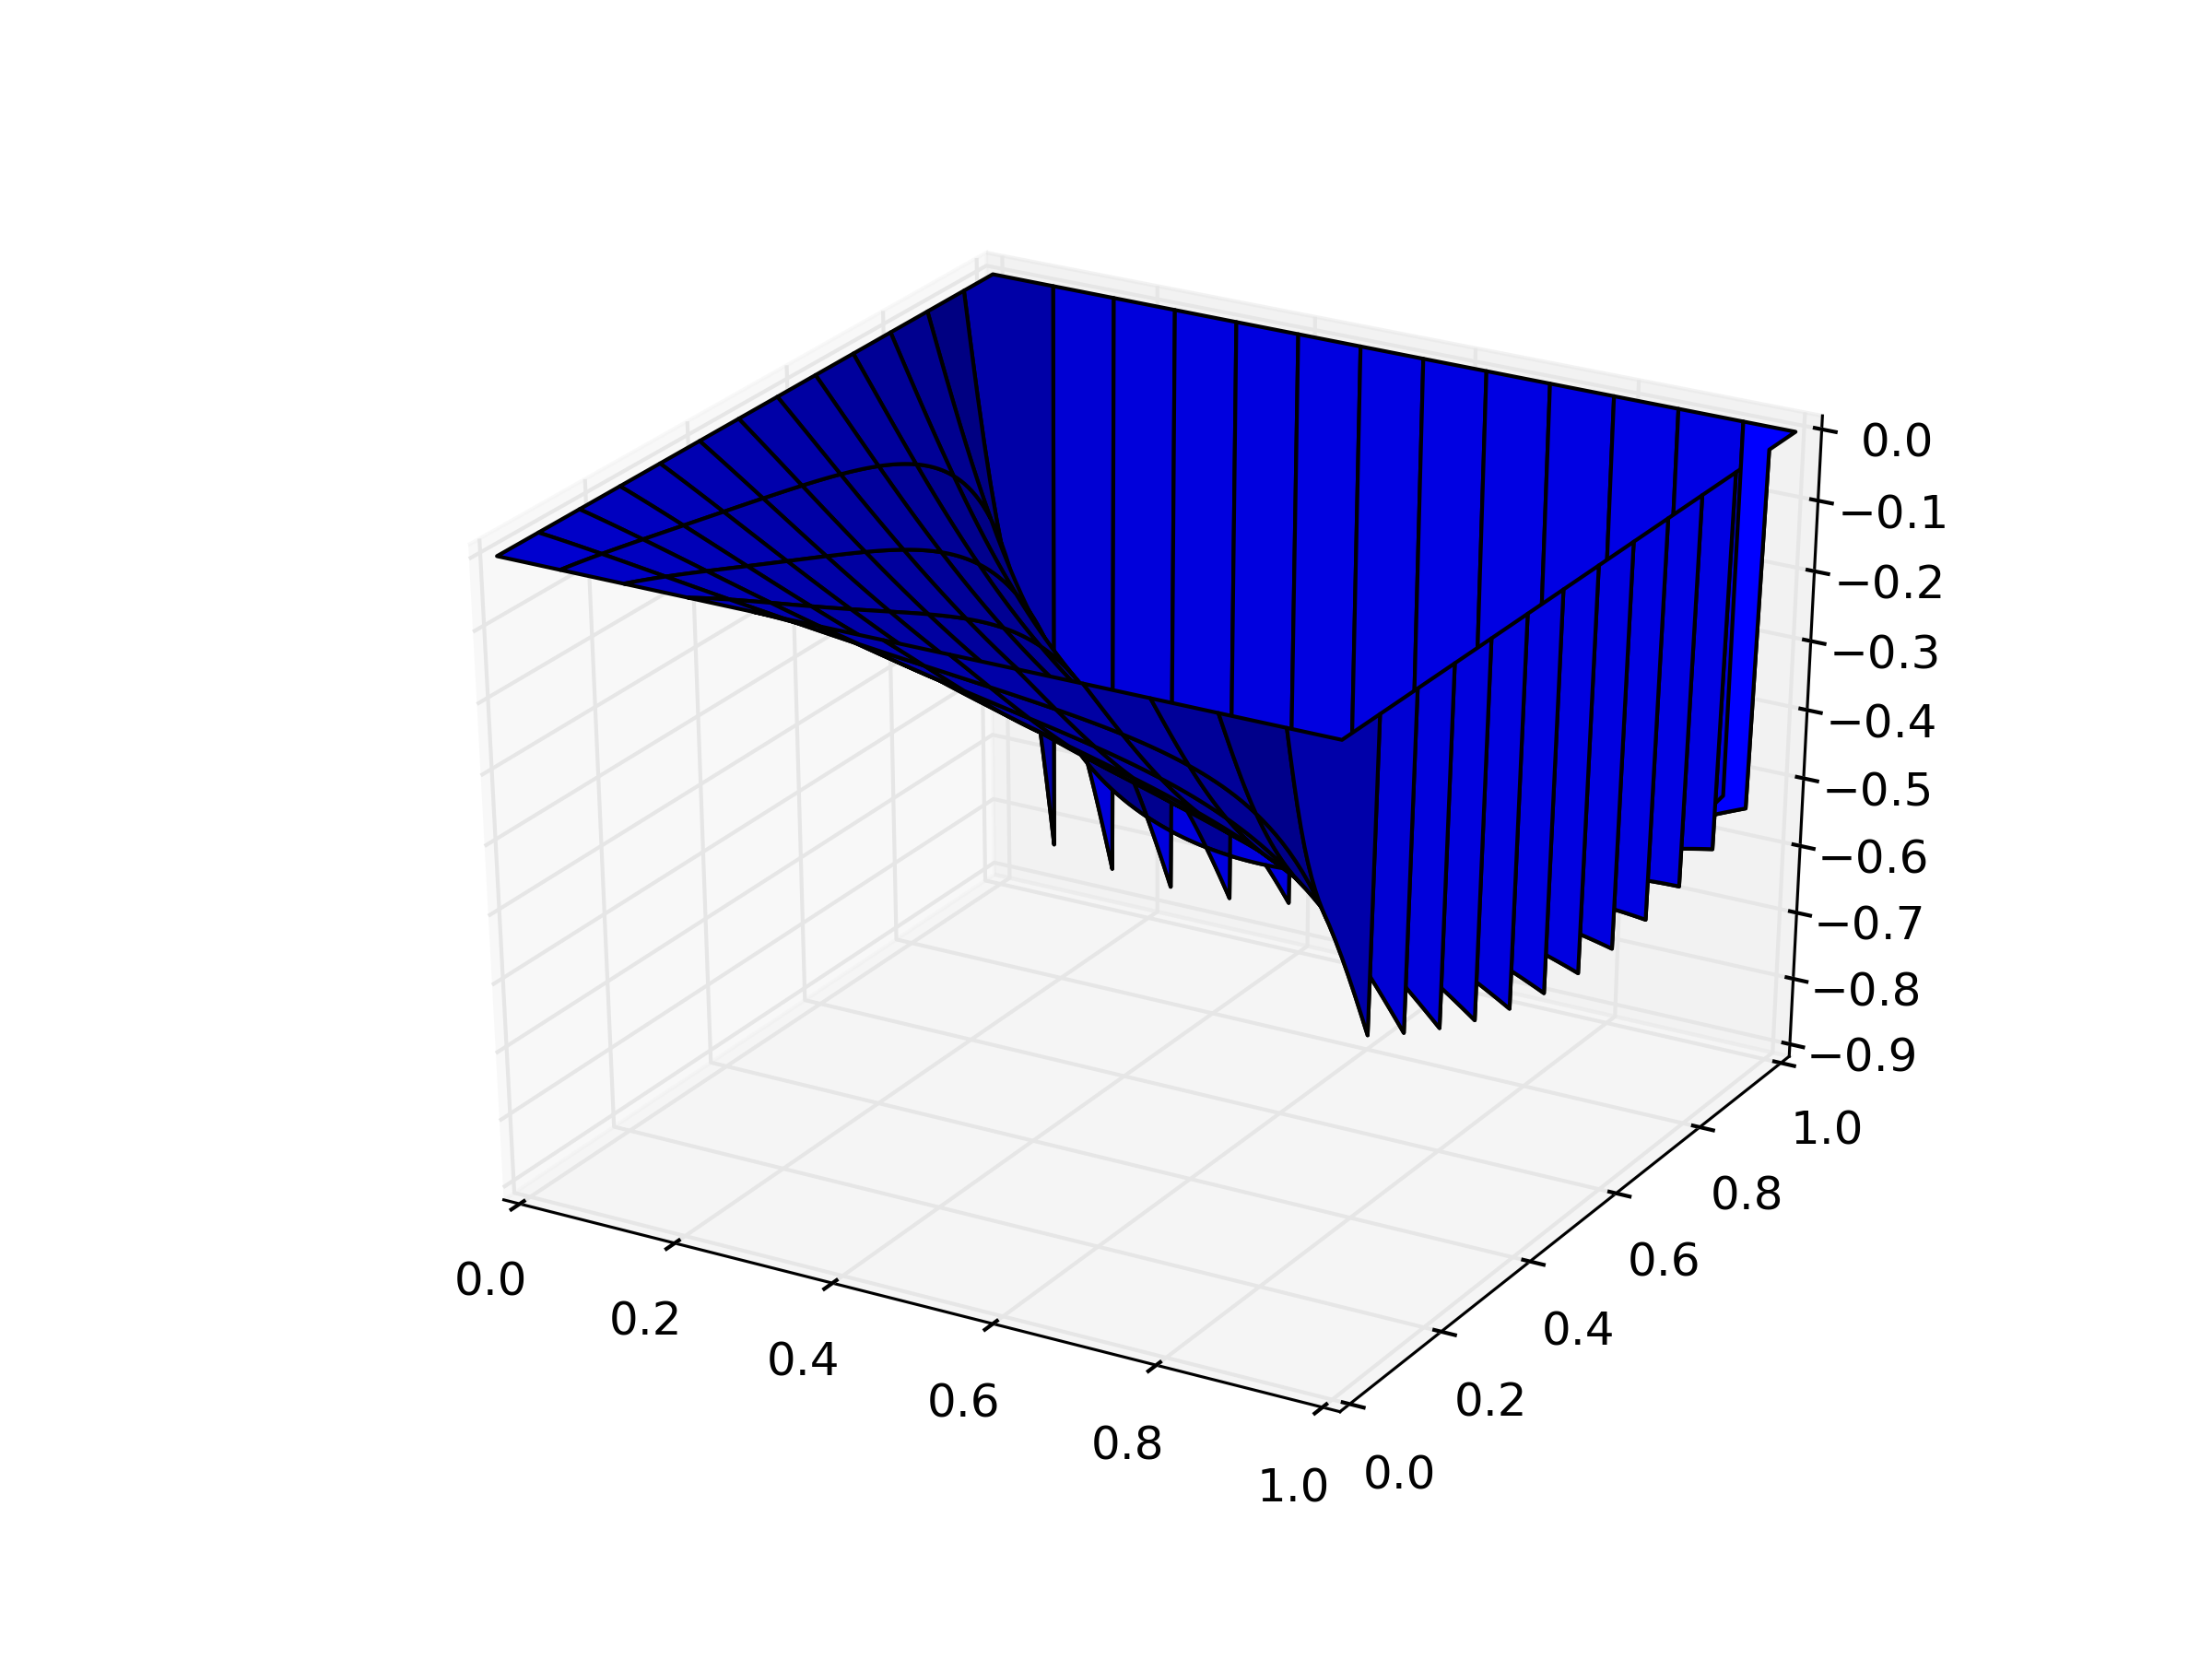
\includegraphics[width=0.3\textwidth]{figure_1_gs_2.png}
    \end{figure}
    \FloatBarrier
    The number of iterations required to have a relative error less than $0.0001$ (that is, $\norm{u^{k+1} - u^k}_1 < \E\norm{u_k}_1$, where $\E = 0.0001$) is
    \begin{align*}
        \begin{array}{||l|l|l|l||}\hline\hline
            h & \text{iterations} & \text{multiplicative factor} & \text{time taken (in seconds)}\\[.1cm]\hline\hline
            2^{-5} & 452 & & 1.144104 \\[.1cm]\hline
            2^{-6} & 1319 & 2.92 & 13.163329 \\[.1cm]\hline
            2^{-7} & 3121 & 2.37 & 123.097511 \\[.1cm]\hline\hline
        \end{array}
    \end{align*}
    Here is a graph of the relative errors as a function of the iteration number:
    \begin{figure}[ht!]
        \centering
        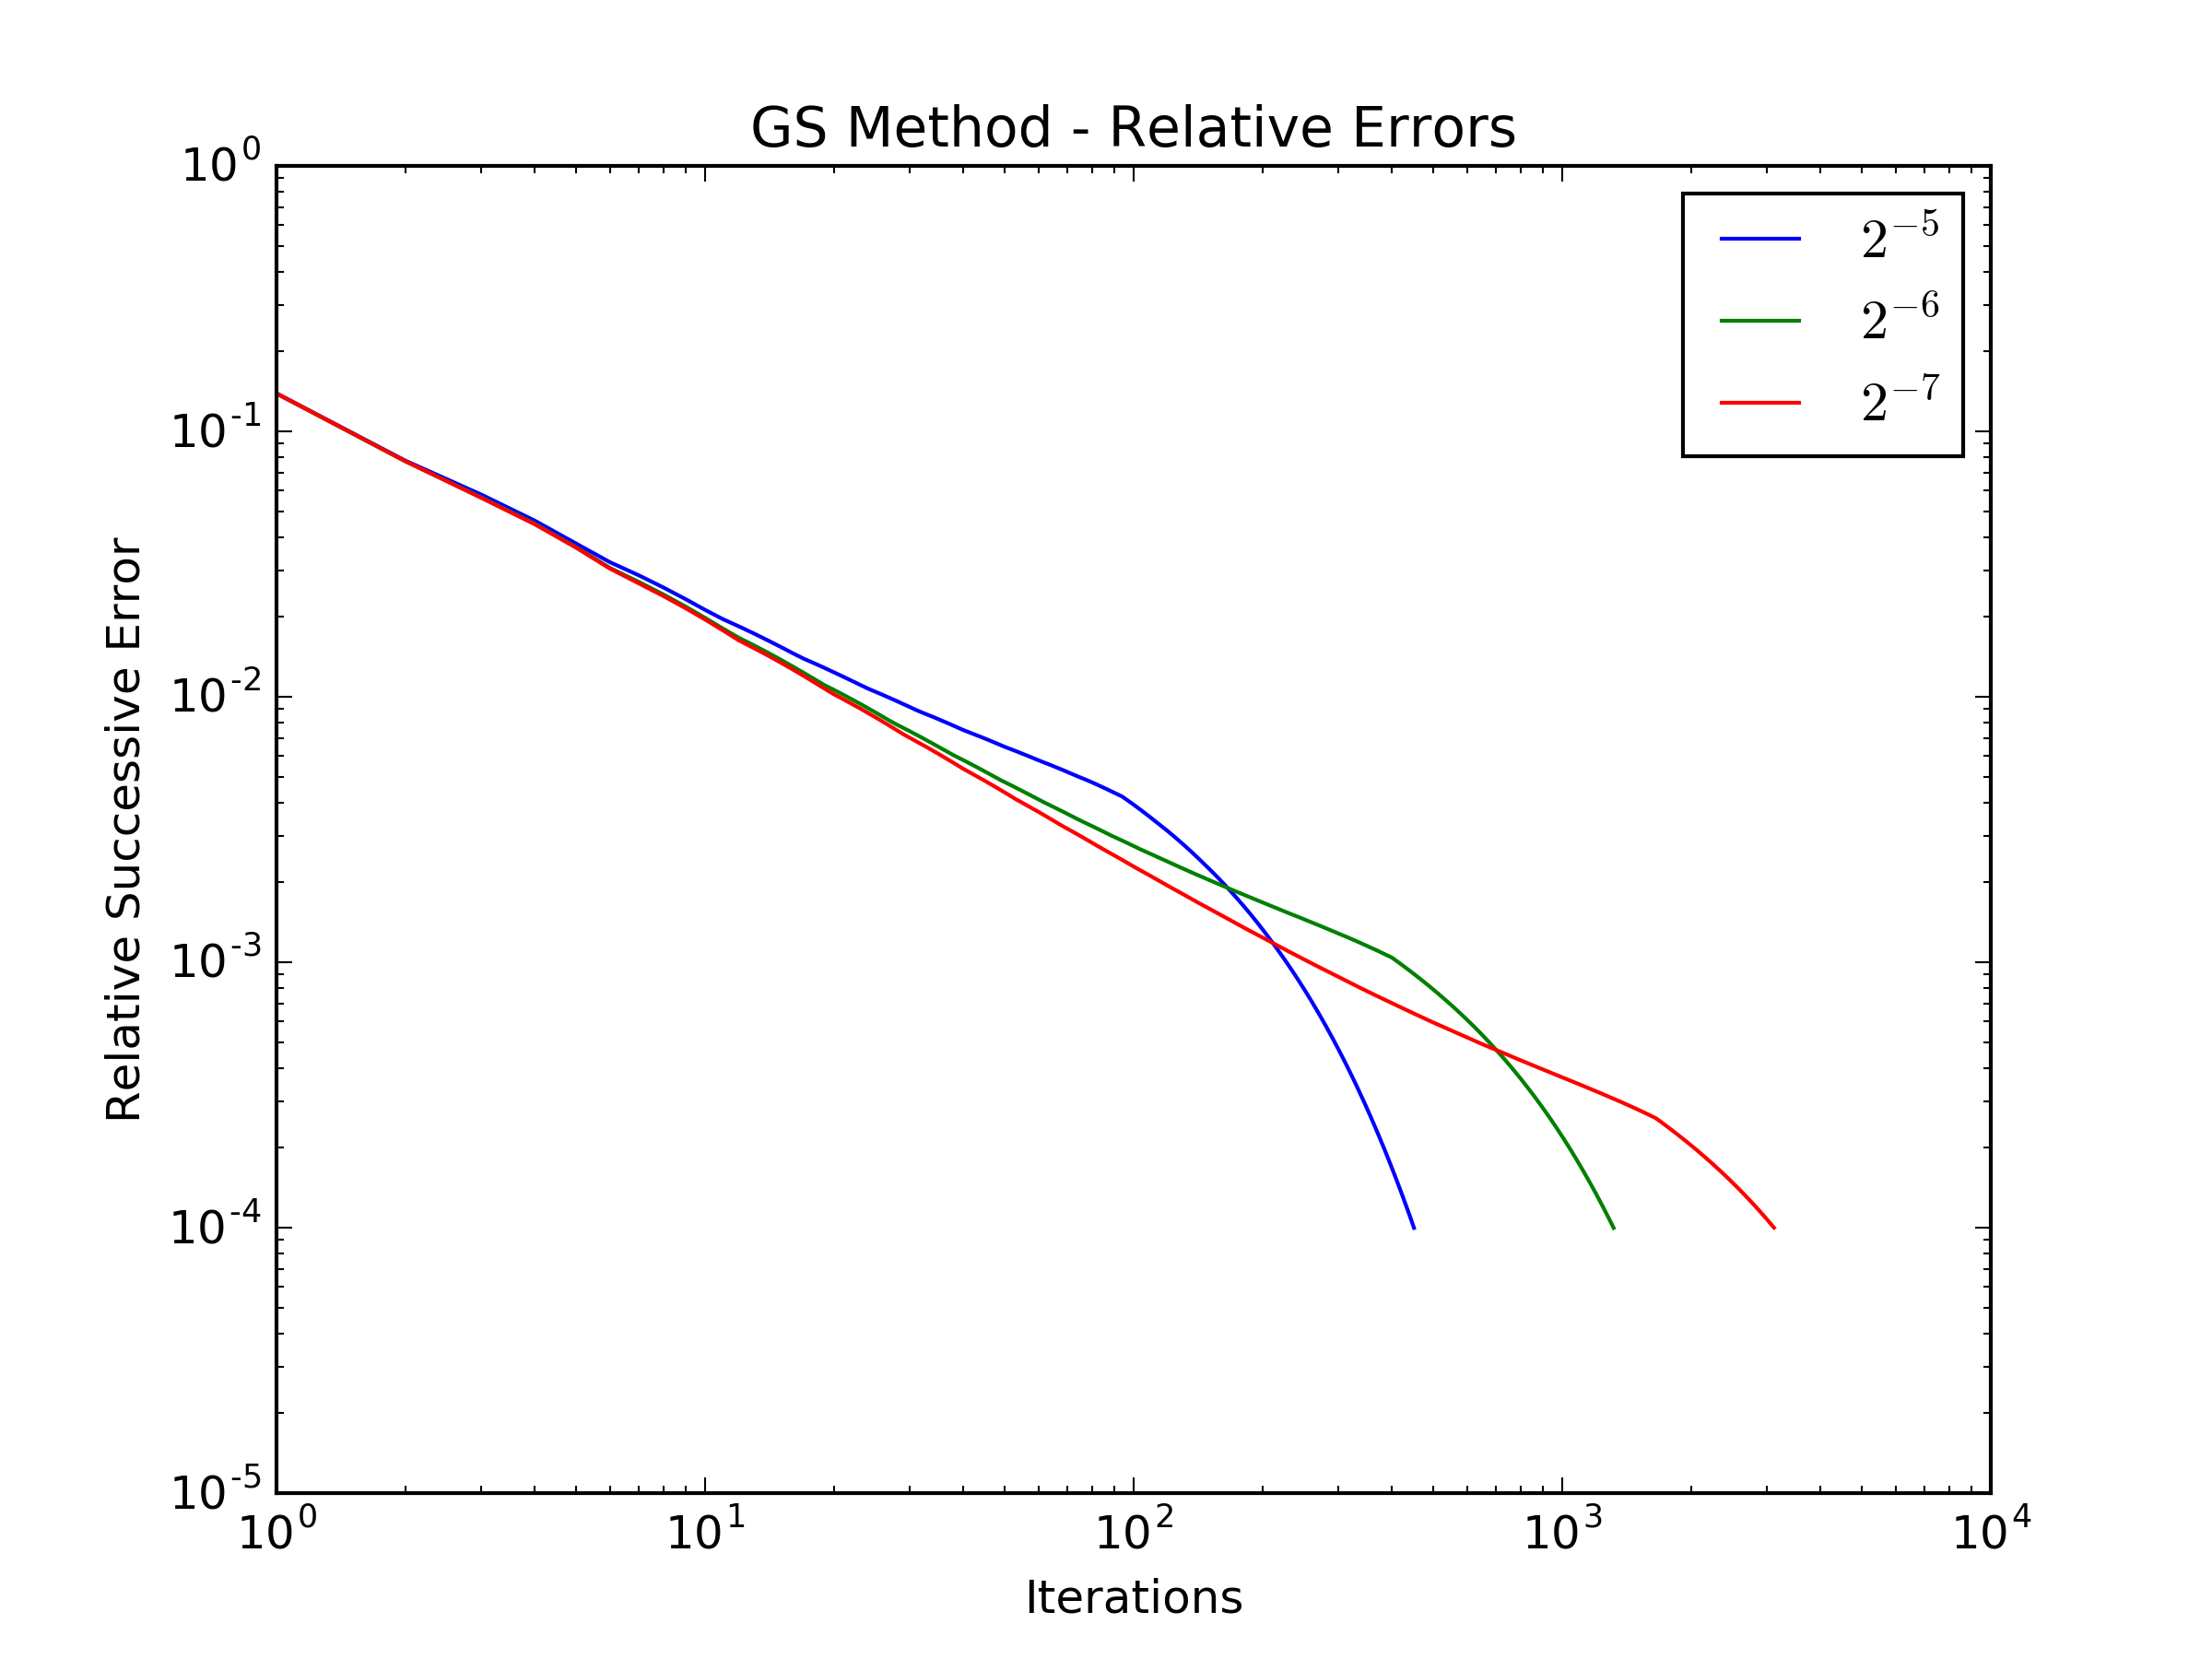
\includegraphics[width=0.5\textwidth]{figure_1_error_gs.png}
    \end{figure}
    \FloatBarrier
    \item SOR
    \begin{align*}
        u_{i,j}^{k+1} = \frac{\omega}{4}\qty(u_{i-1,j}^k + u_{i+1,j}^k + u_{i,j-1}^k + u_{i,j+1}^k - h^2f_{i,j}) + (1 - \omega)u_{i,j}^k
    \end{align*}
    where $\omega$ is the optimal $\omega$ for convergence, i.e.
    \begin{align*}
        \omega = \omega^* = 2(1 - \pi h).
    \end{align*}
    Here are the results for $h = 2^{-i}$ for $i=5,6,7$.
    \begin{figure}[ht!]
        \centering
        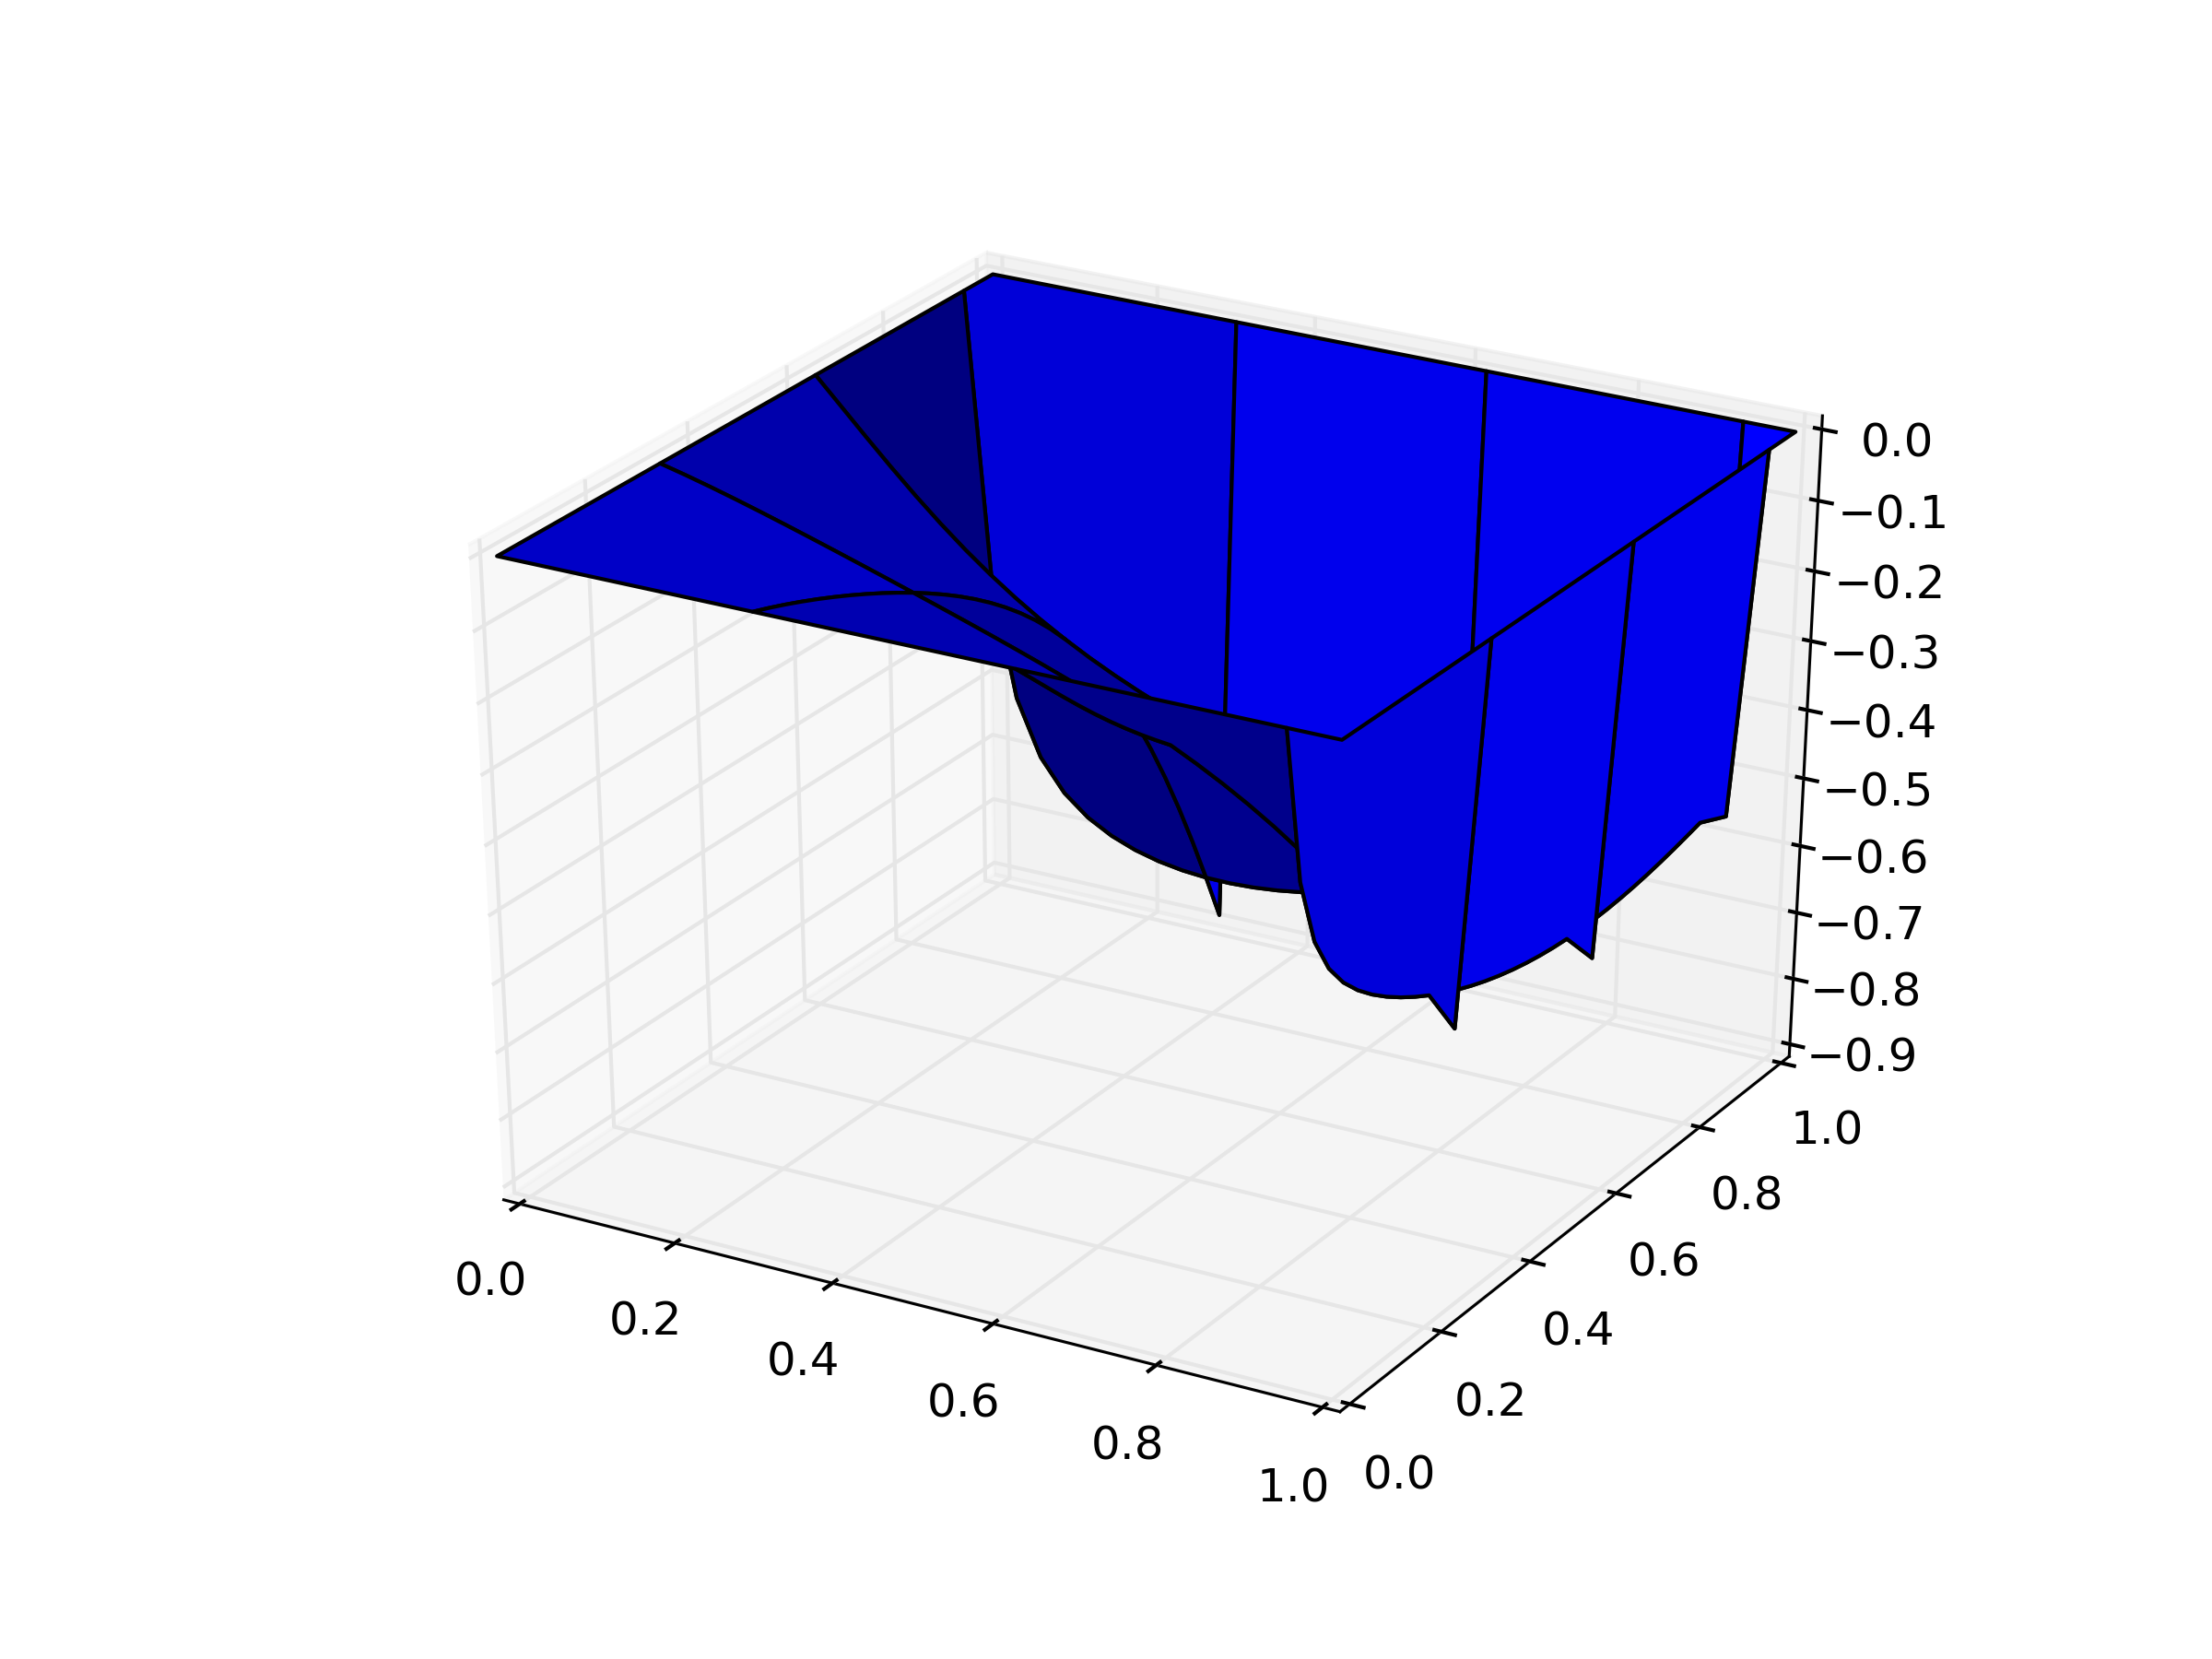
\includegraphics[width=0.3\textwidth]{figure_1_sor_0.png}
        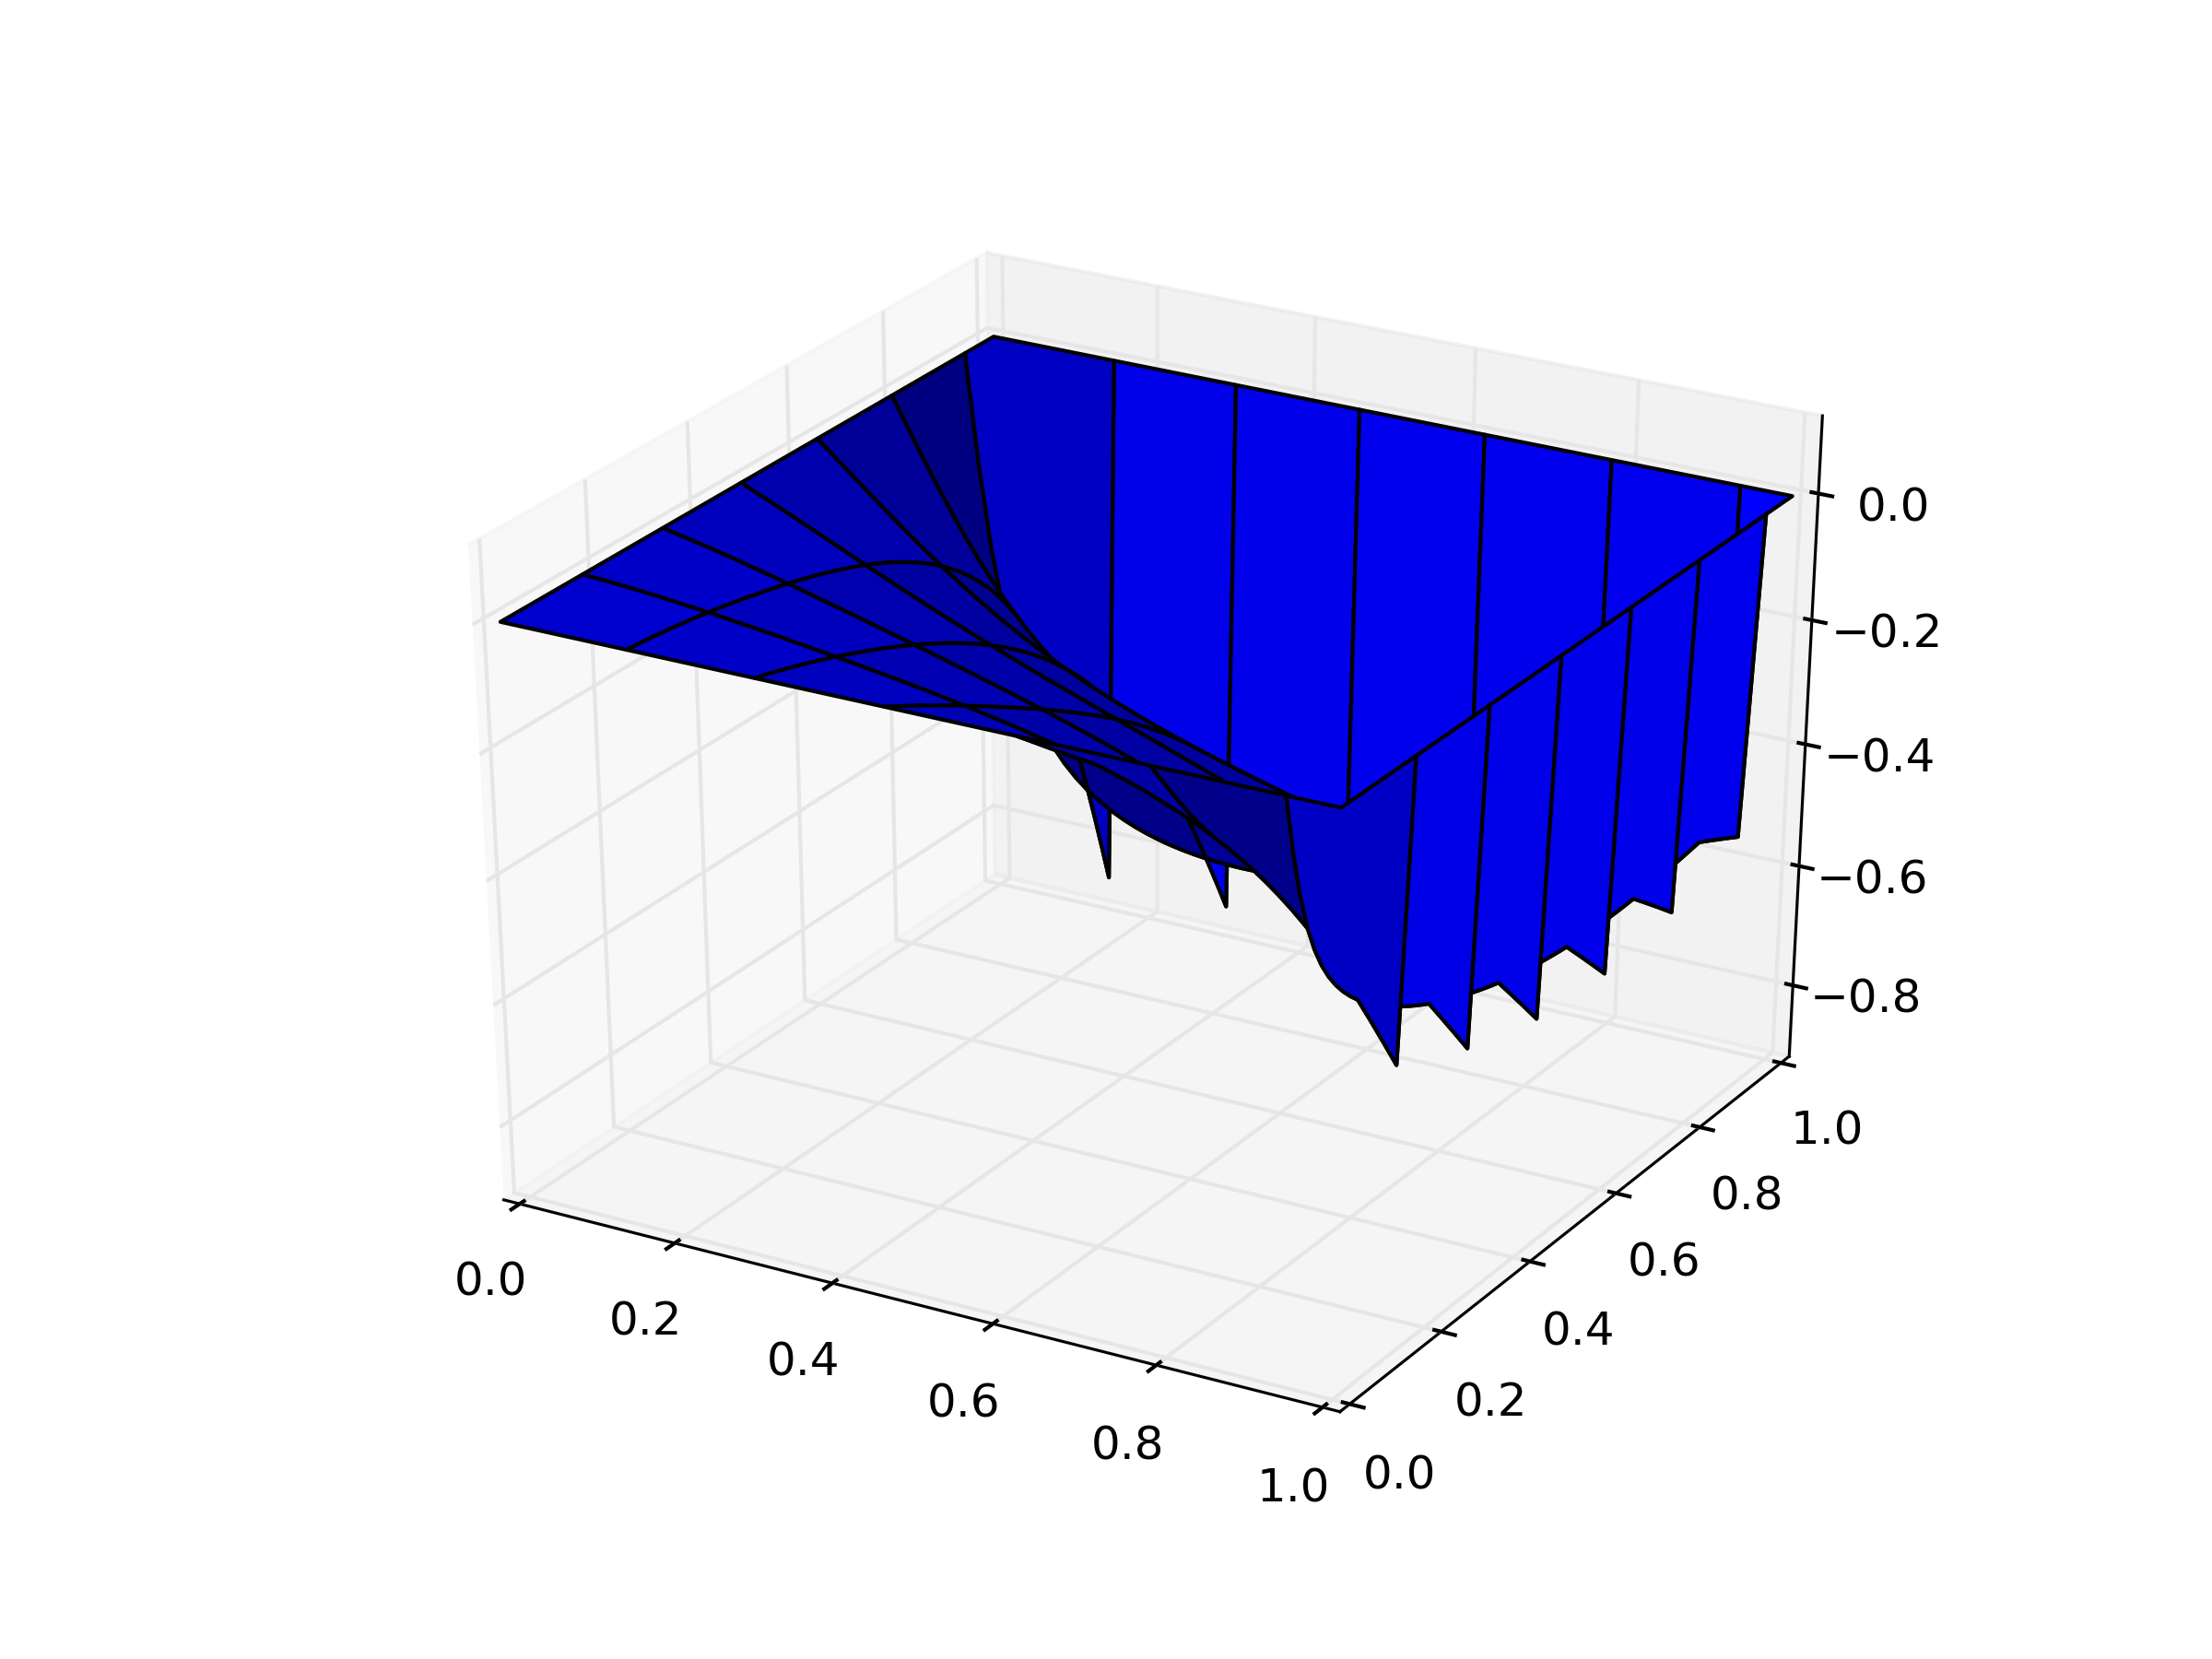
\includegraphics[width=0.3\textwidth]{figure_1_sor_1.png}
        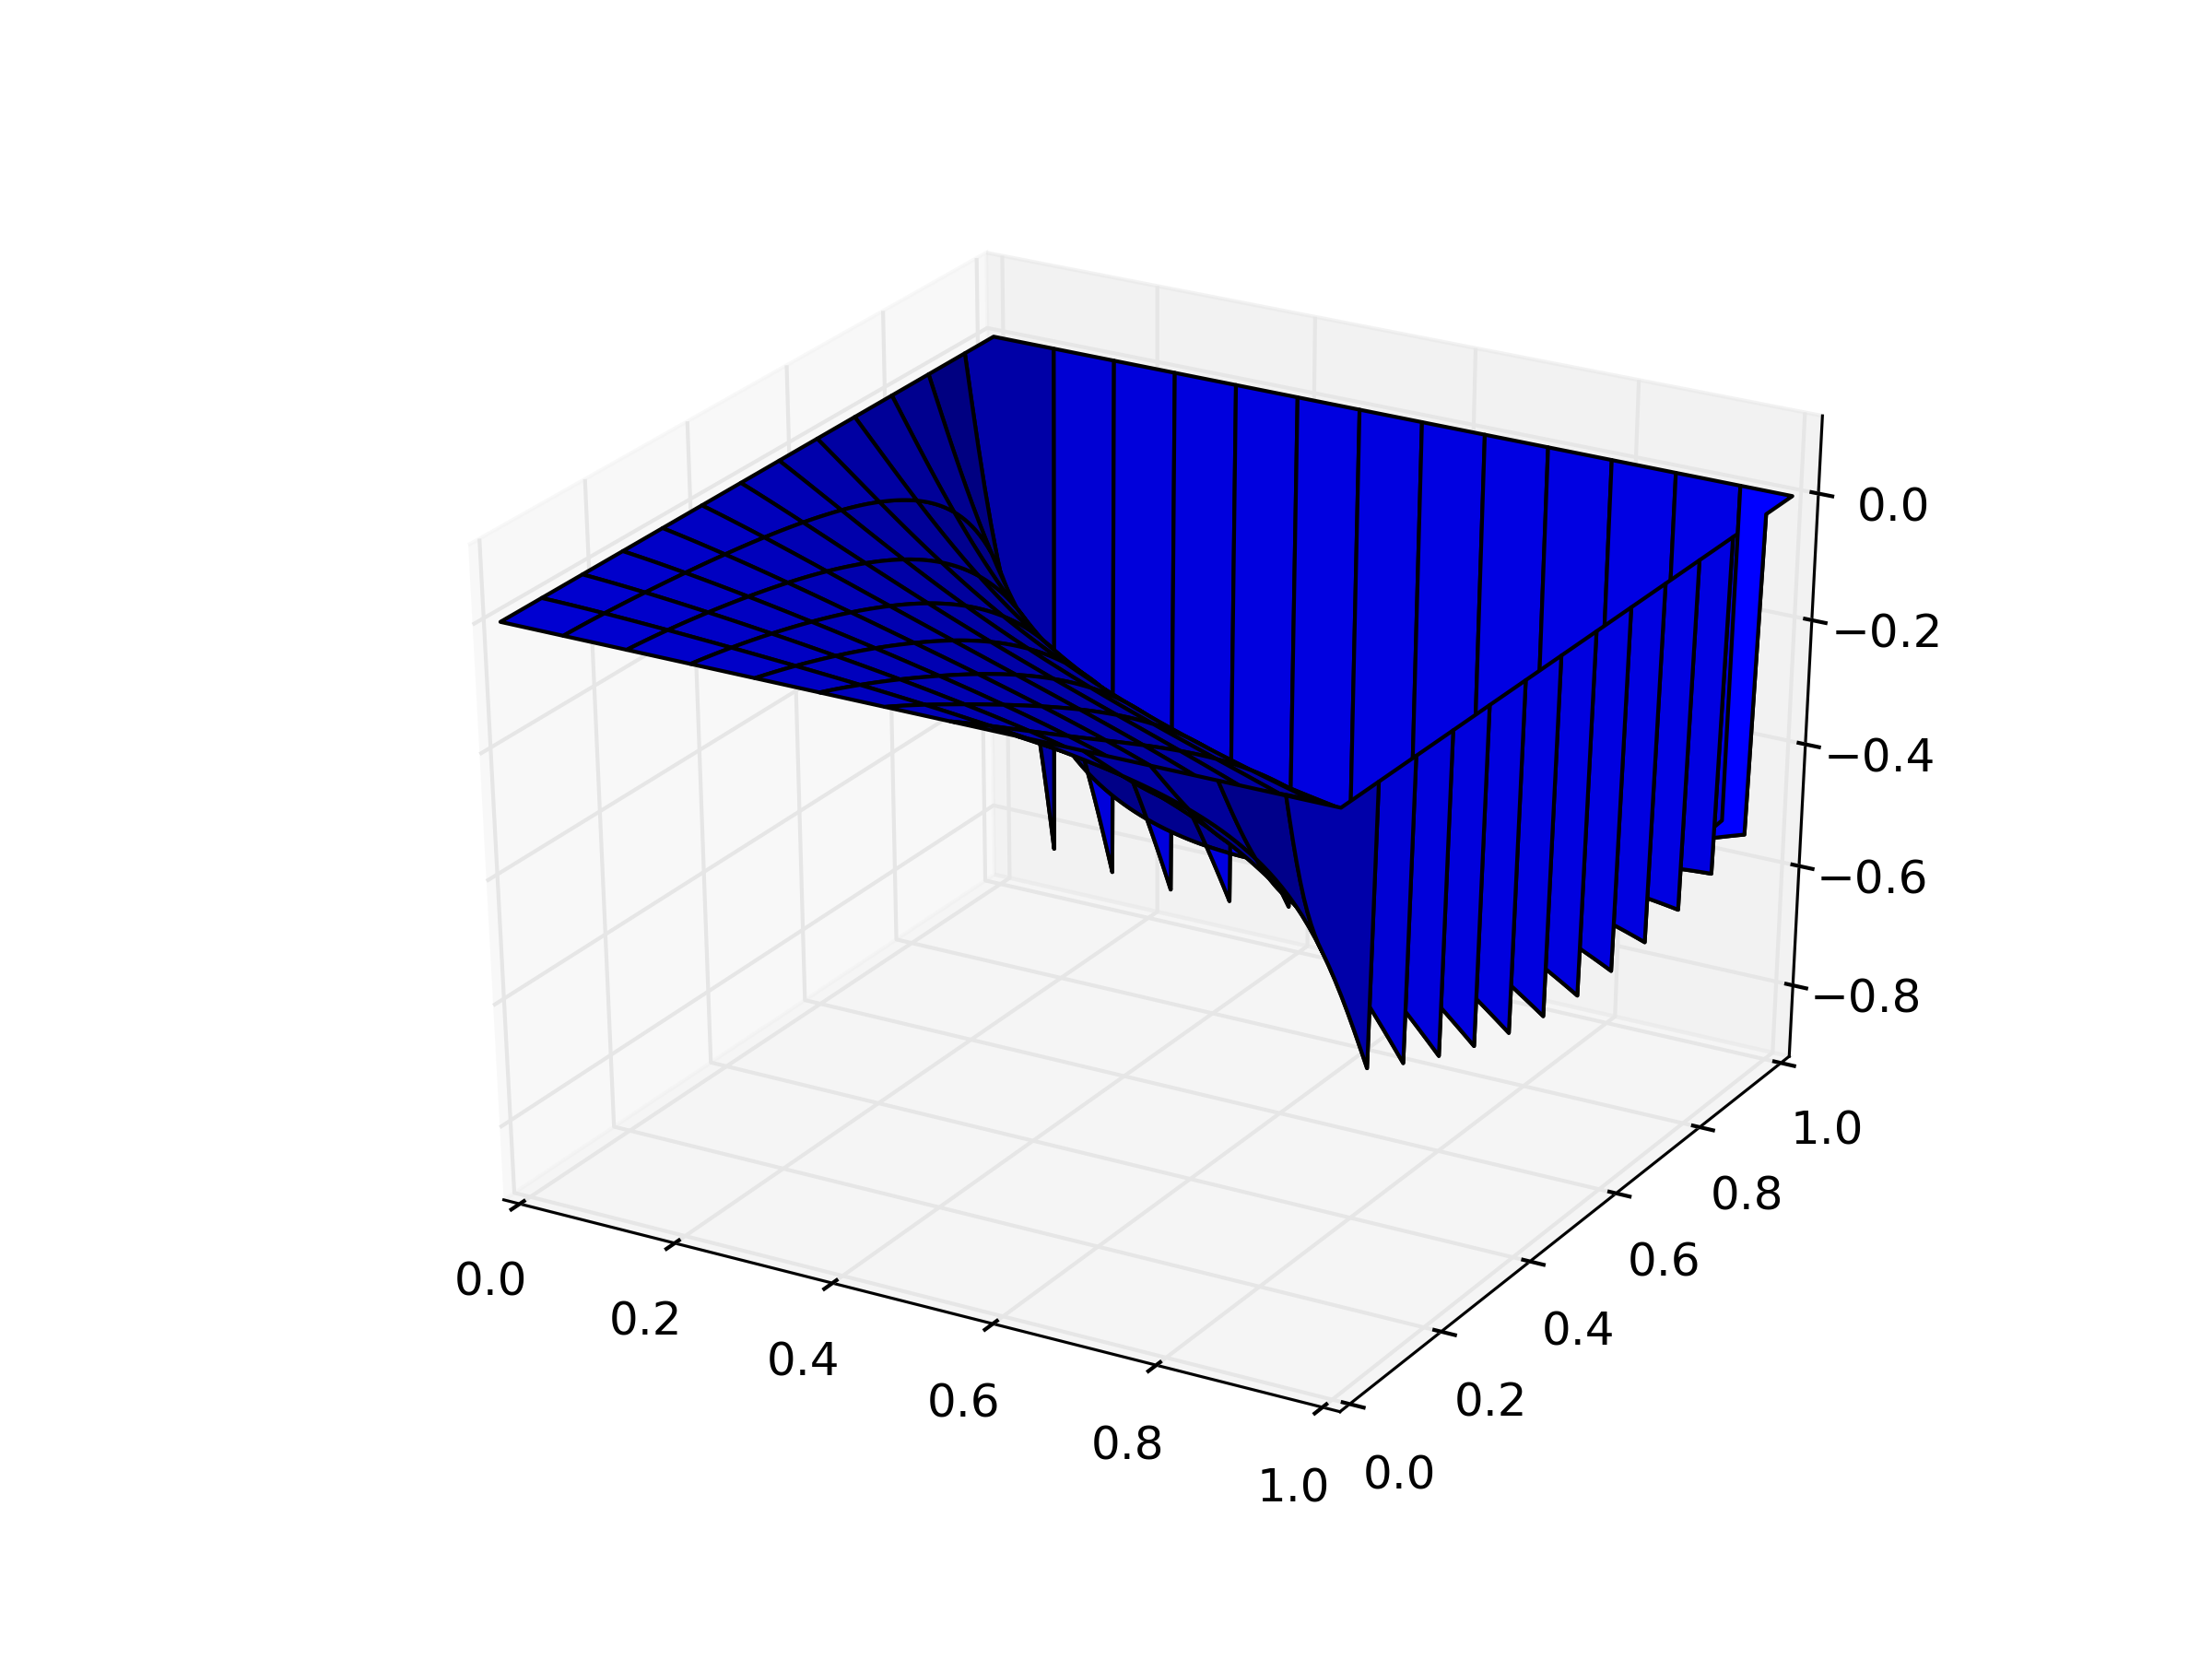
\includegraphics[width=0.3\textwidth]{figure_1_sor_2.png}
    \end{figure}
    \FloatBarrier
    The number of iterations required to have a relative error less than $0.0001$ (that is, $\norm{u^{k+1} - u^k}_1 < \E\norm{u_k}_1$, where $\E = 0.0001$) is
    \begin{align*}
        \begin{array}{||l|l|l|l||}\hline\hline
            h & \text{iterations} & \text{multiplicative factor} & \text{time taken (in seconds)} \\[.1cm]\hline\hline
            2^{-5} & 58 & & 0.181905 \\[.1cm]\hline
            2^{-6} & 100 & 1.72 & 1.148622 \\[.1cm]\hline
            2^{-7} & 177 & 1.77 & 8.517767 \\[.1cm]\hline\hline
        \end{array}
    \end{align*}
    Here is a graph of the relative errors as a function of the iteration number:
    \begin{figure}[ht!]
        \centering
        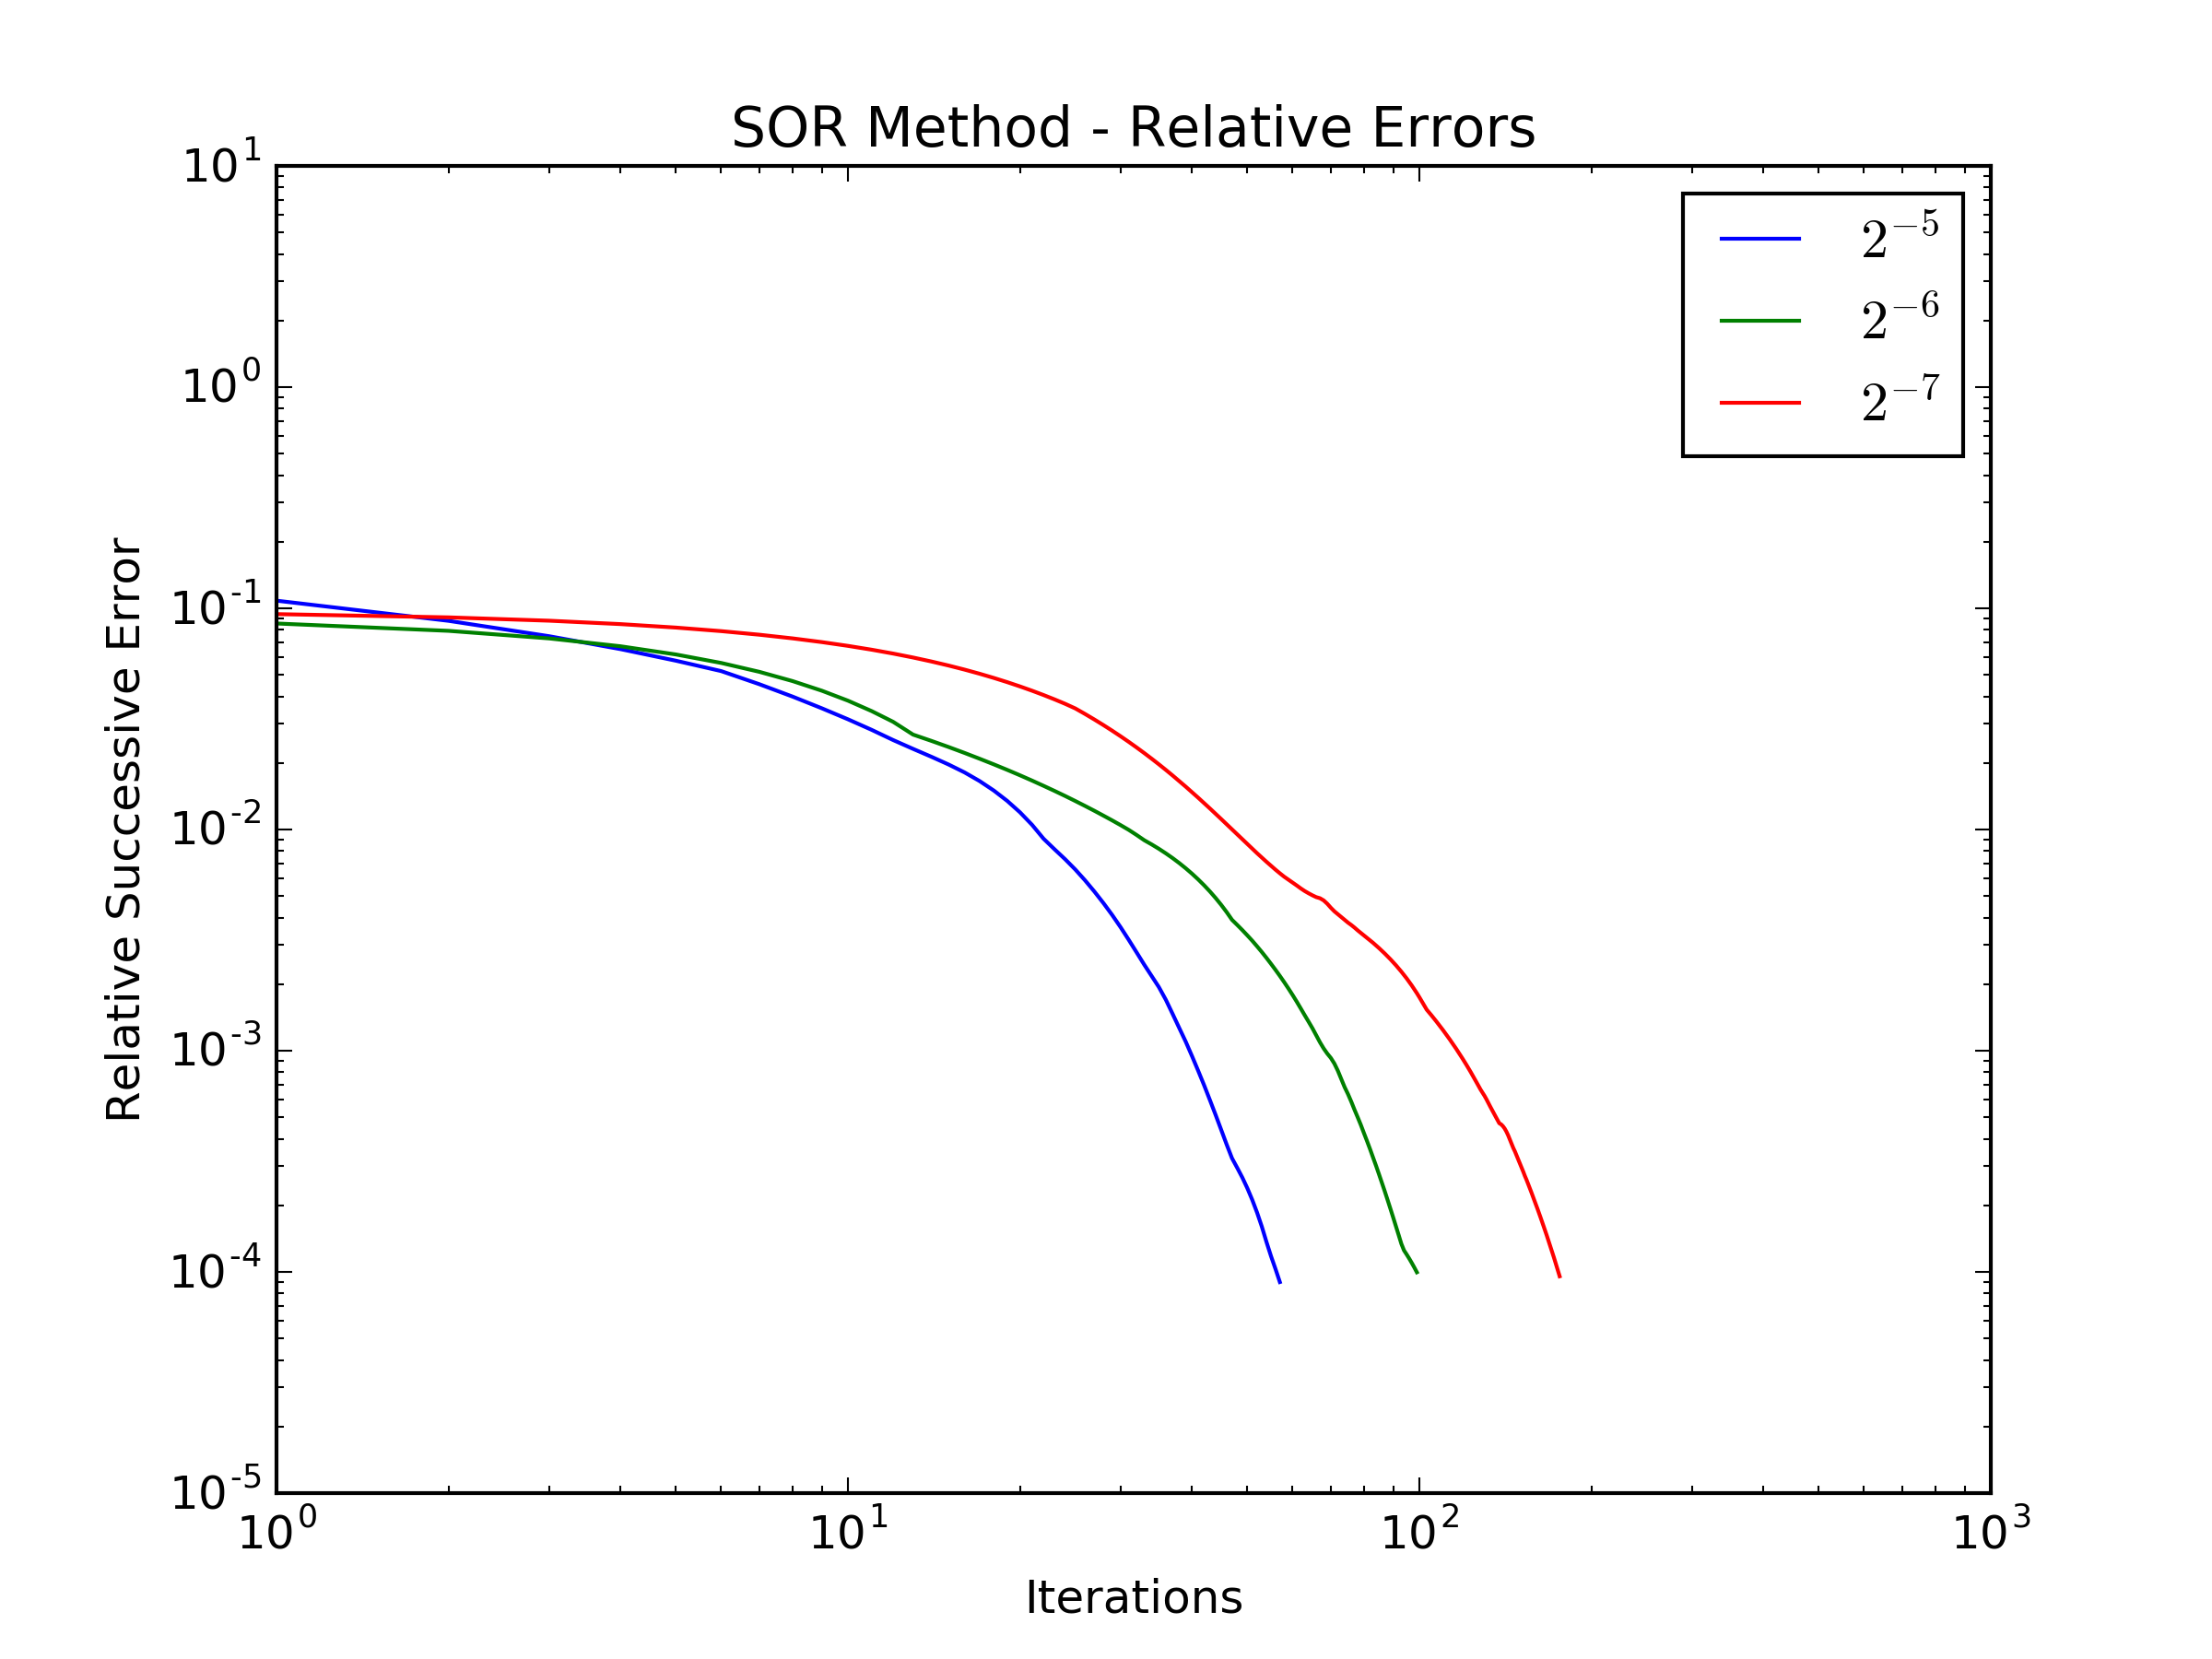
\includegraphics[width=0.5\textwidth]{figure_1_error_sor.png}
    \end{figure}
    \FloatBarrier
\end{itemize}









\problem{Problem 2}{When solving parabolic equations numerically, one frequently needs to solve an equation of the form $$u - \delta\laplacian u = f,$$ where $\delta > 0$.  The analysis and numerical methods we have discussed for the Poisson equation can be applied to the above equation.  Suppose we are solving the above equation on the unit square with Dirichlet boundary conditions.  Use the standard five point stencil for the discrete Laplacian.
\begin{enumerate}[\ \ (a)]
    \item Analytically compute the eigenvalues of the Jacobi iteration matrix, and show that the Jacobi iteration converges.
    \item If $h = 10^{-2}$ and $\delta = 10^{-4}$, how many iterations of SOR would it take reduce the error by a factor of $10^{-6}$?  How many iterations would it take for the Poisson equation?  Use that the spectral radius of SOR is $$\rho_\text{SOR} = \omega_\text{opt} - 1,$$ where $$\omega_\text{opt} = \frac{2}{1 + \sqrt{1 - \rho_J^2}},$$ and where $\rho_J$ is the spectral radius of Jacobi.
\end{enumerate}
}

\begin{enumerate}[\ \ (a)]
    \item
        \begin{align*}
            u - \delta\laplacian u &= f \\
            (I - \delta A)u &= f
        \end{align*}
        but $I - \delta A = D - L - U$, so $L + U = D - I + \delta A$, thus
        \begin{align*}
            (I - \delta A)u &= f \\
            (D - L - U)u &= f \\
            Du &= (L + U)u + f \\
            u &= (I - D^{-1}\qty(I - \delta A))u + D^{-1}f \\
            &= Tu + C
        \end{align*}
        where
        \begin{align*}
            T = (I - D^{-1}\qty(I - \delta A)) \qquad \text{and} \qquad C = D^{-1}f
        \end{align*}
        We know the eigenvalues of $A$ are
        \begin{align*}
            \mu_{ij} = \frac{2}{h^2}\cos(\ell\pi h) + \cos(j\pi h) - 2,
        \end{align*}
        so the eigenvalues of $I - \delta A$ are $1 - \delta \mu_{ij}$, and the eigenvalues of $I - D^{-1}\qty(I - \delta A)$ are
        \begin{align*}
            \tilde{\mu}_{ij} = 1 - \frac{1}{1 + \dfrac{4\delta}{h^2}}\qty(1 - \delta \mu_{ij})
        \end{align*}
        since
        \begin{align*}
            D = \qty[\begin{array}{cccc}
                1 + \dfrac{4\delta}{h^2} & 0 & \dots & 0 \\
                0 & 1 + \dfrac{4\delta}{h^2} & \dots & 0 \\
                \vdots & \vdots & \ddots & \vdots \\
                0 & 0 & \dots & 1 + \dfrac{4\delta}{h^2}
            \end{array}]
        \end{align*}
        Thus, after simplification,
        \begin{align*}
            \tilde{\mu}_{ij} = \frac{2\delta}{h^2 + 4\delta}\qty(\cos(\ell\pi h) + \cos(j\pi h))
        \end{align*}

        To prove convergence, the largest eigenvalue is found by setting $\ell = j = 1$, and thus
        \begin{align*}
            \tilde{\mu}_{ij} = \frac{4\delta}{h^2 + 4\delta}\qty(\cos(\pi h)) < 1.
        \end{align*}
        Since the largest eigenvalue is less than one, the iterative scheme must converge.
    \item
        The spectral radius $\rho_J$ is given by
        \begin{align*}
             \rho_J = \displaystyle\max_{i,j}\tilde{\mu}_{ij} = \frac{4\delta}{h^2 + 4\delta}\cos(\pi h)
        \end{align*}
        For $\delta = 10^{-4}$ and $h = 10^{-2}$, we have
        \begin{align*}
            \rho_J \approx 0.7996
        \end{align*}
        which gives
        \begin{align*}
            \omega_\text{opt} = \frac{2}{1 + \sqrt{1 - \rho_J^2}} \approx 1.2496
        \end{align*}
        and thus
        \begin{align*}
            \rho_\text{SOR} \approx 0.2496.
        \end{align*}
        So for SOR, to guarantee the error is reduced by a factor of $10^{-6}$, set the number of iterations $k$ such that
        \begin{align*}
            \rho_\text{SOR}^k &= 10^{-6} \\
            \implies k = \frac{\log(10^{-6})}{\log(\rho_\text{SOR})} &\approx 10,
        \end{align*}
        that is, we need 10 iterations to guarantee a $6$th order reduction in error.  For the Poisson equation, set $\rho_J = \cos(\pi h)$ where $h = 10^{-2}$, thus $\omega_\text{opt} \approx 1.9391$ and so $\rho_\text{Poisson} \approx 0.9391$.  Then
        \begin{align*}
            k = \frac{\log(10^{-6})}{\log(\rho_\text{Poisson})} \approx 220,
        \end{align*}
        that is, we need 220 iterations to guarantee a $6$th order reduction in error.
\end{enumerate}











\problem{Problem 3}{In this problem we compare the speed of SOR to a direct solve using Gaussian elimination.  At the end of this assignment is MATLAB code to form the matrix for the 2D discrete Laplacian.  The code for the 3D matrix is similar.  Note that with 1 GB of memory, you can handle grids up to about $1000\times1000$ in 2D and $40\times40\times40$ in 3D with a direct solve.  The range of grids you will explore depends on the amount of memoery you have.
\begin{enumerate}[\ \ (a)]
    \item Solve the PDE from problem 1 using a direct solve.  Put timing commands in your code and report the time to solve for a range of mesh spacings.  Use SOR to solve on the same meshes and report the time and number of iterations.  Comment on your results.  Note that the timing results depend strongly on your implementation.  Comment on the efficiency of your program.
    \item Repeat the previous part in three spatial dimensions for a range of mesh spacings.  Change the right side of the equation to be a three dimensional Gaussian.  Comment on your results.
\end{enumerate}
}

\begin{enumerate}[\ \ (a)]
    \item
        Using the penta-diagonal matrix for 2D Laplacian with Dirichlet boundary conditions,
        \begin{align*}
            A = \qty[\begin{array}{ccccccccccccccccccc} 0 & 0 & \dots & 0 & 1 & 0 \dots & 0 & 1 & -4 & 1 & 0 & \dots & 0 & 1 & 0 & \dots & 0 & 0
            \end{array}],
        \end{align*}
        where there are $1$s on the first and $N$th super-~and sub-diagonals, and $-4$ on the diagonal, here are the results of using a direct solve method (python's sparse matrix solver) vs.~my implementation of the SOR method (tolerance$=0.001$):
        \begin{align*}
            \begin{array}{||l|l|l|l|l||}\hline\hline
                h & \text{SOR iterations} & \text{SOR iteration mult.~factor} & \text{SOR time taken (in sec.)} & \text{Direct solve time taken (in sec.)} \\\hline\hline
                2^{-6} & 63 & & 1.091 & 0.01796 \\\hline
                2^{-7} & 117 & 1.857 & 6.418 & 0.08653 \\\hline
                2^{-8} & 210 & 1.795 & 46.421 & 0.55438 \\\hline
                2^{-9} & 403 & 1.919 & 363.982 & 3.69306 \\\hline\hline
            \end{array}
        \end{align*}
        It is abundantly clear my SOR solver is not implemented to its fullest potential.  Here is the graph showing the convergence in relative error for the SOR method:
        \begin{figure}[ht!]
            \centering
            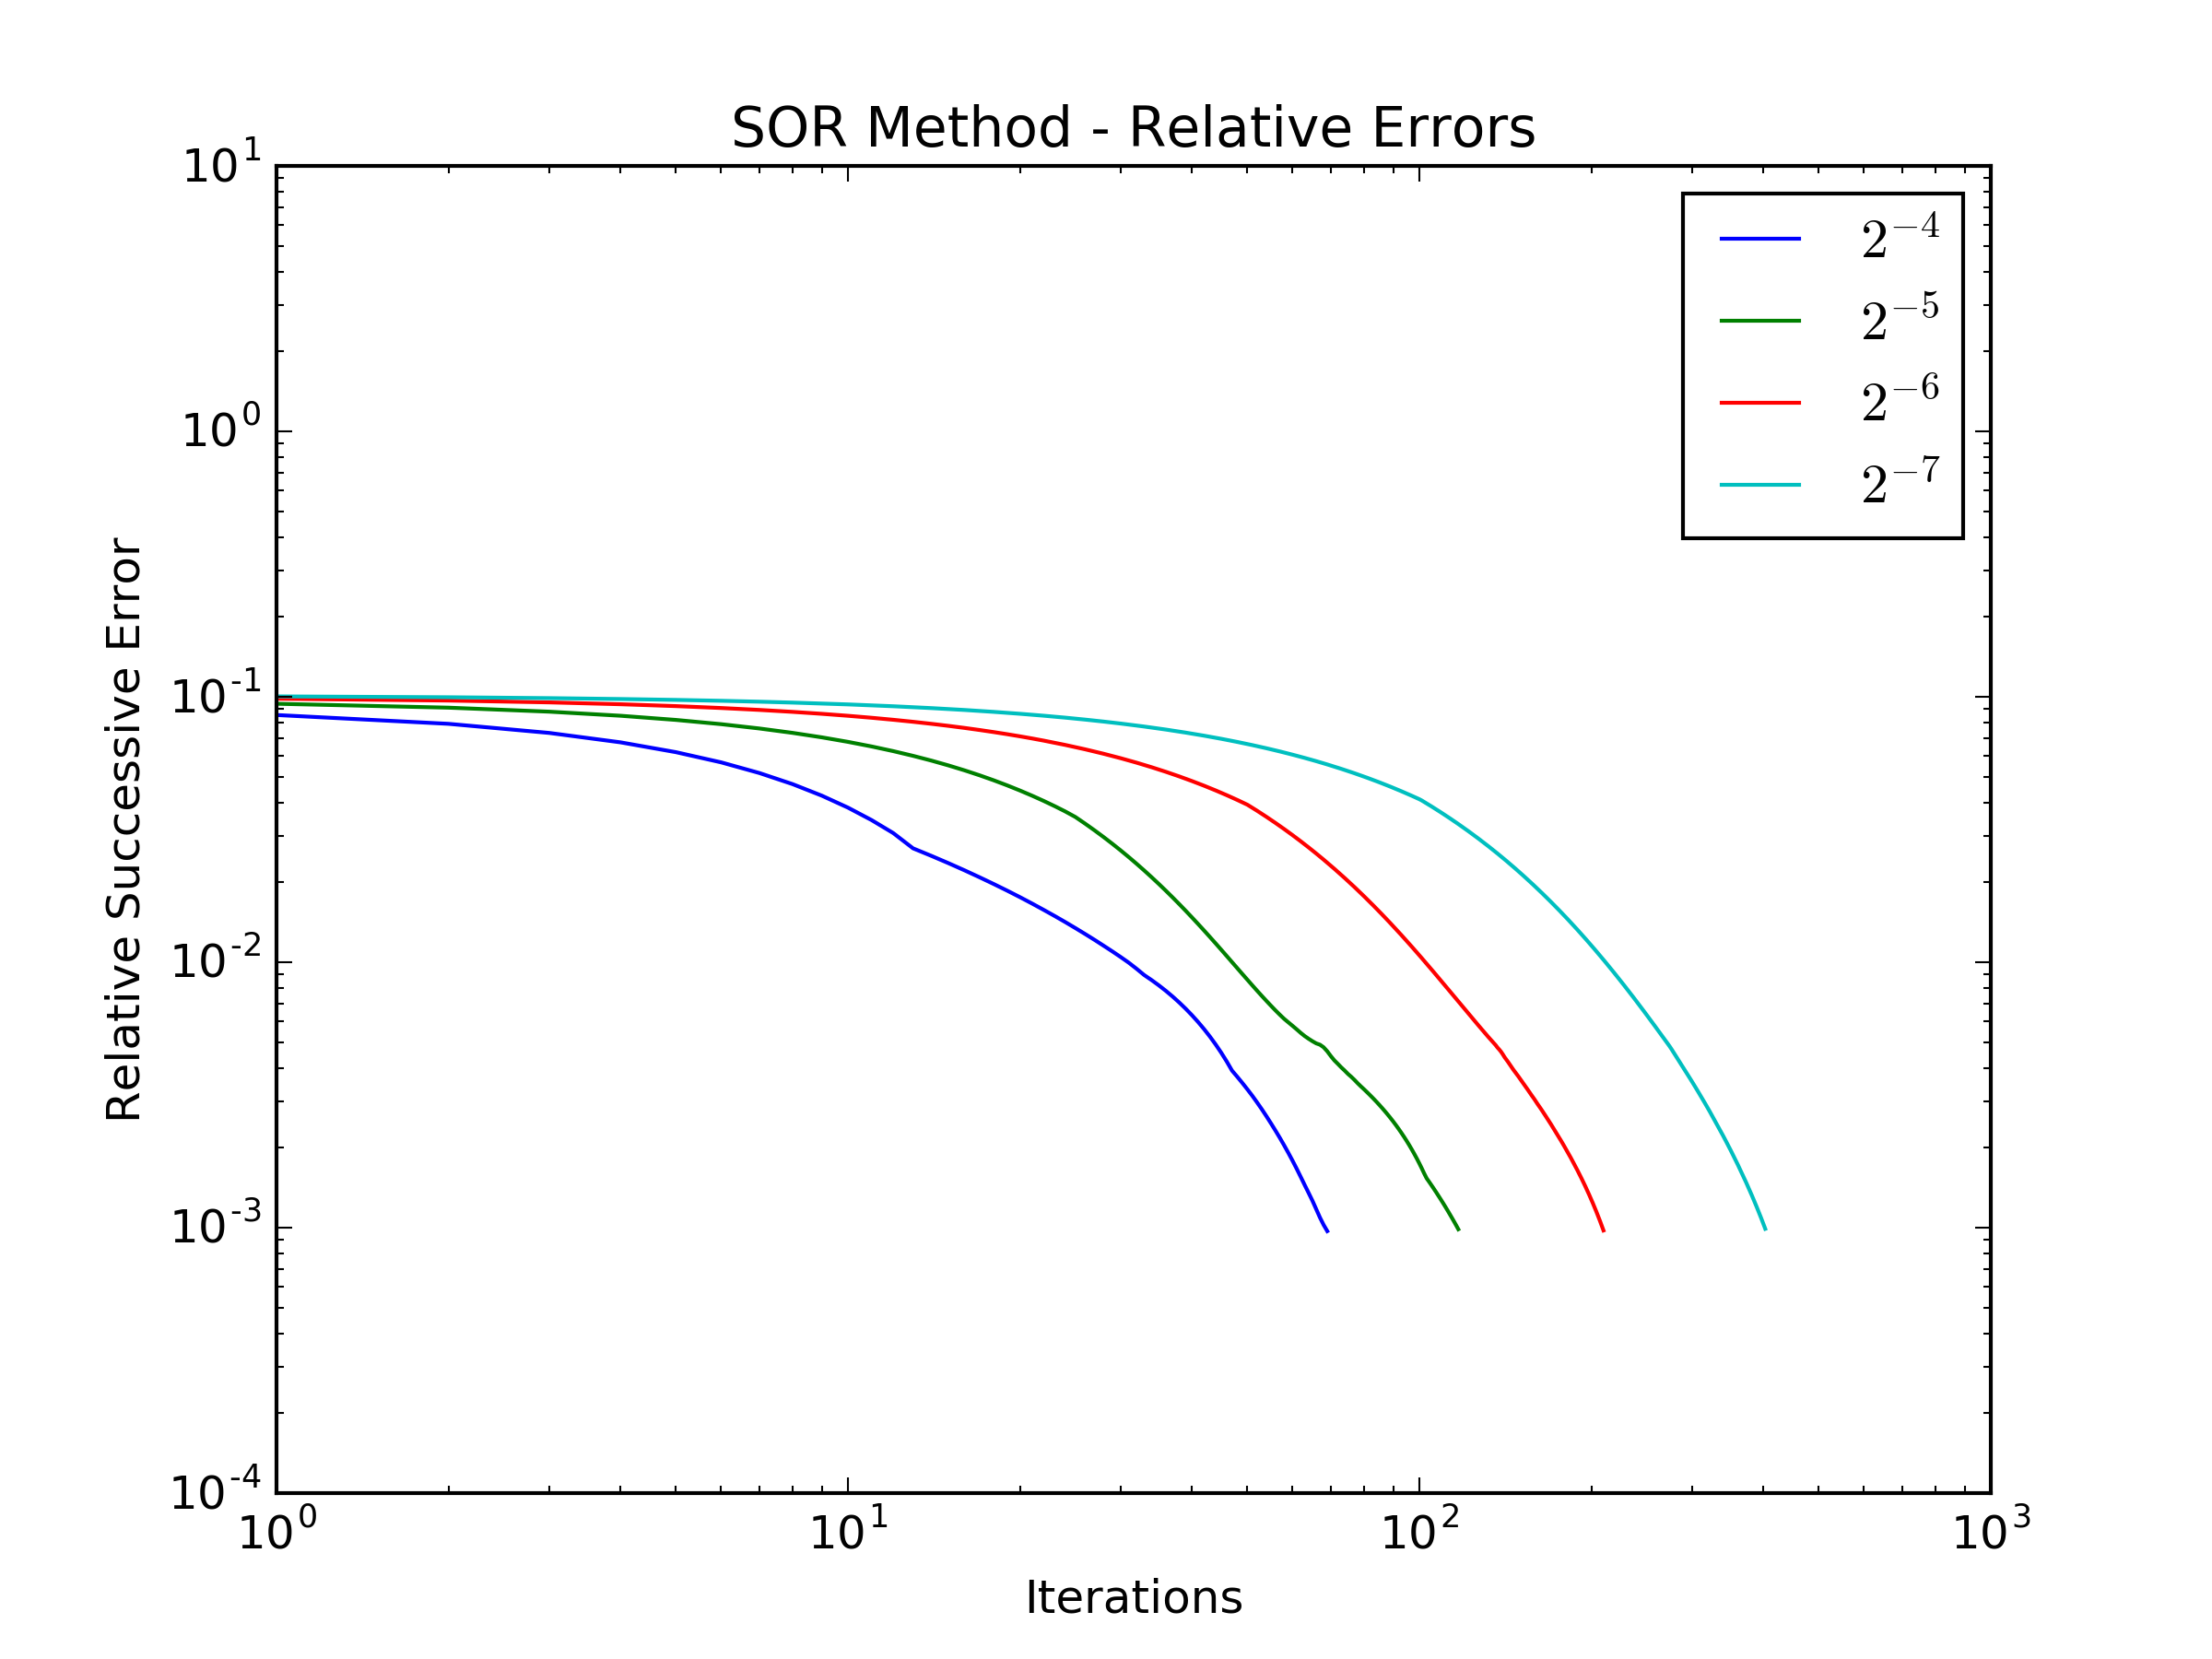
\includegraphics[width=0.5\textwidth]{figure_3_SOR_error_SOR.png}
        \end{figure}
        \FloatBarrier

    \item
        I chose the right hand side to be
        \begin{align}
            f(x,y,z) = -e^{-\qty(x-0.25)^2 - \qty(y - 0.6)^2 - \qty(z - 0.5)^2}
        \end{align}
        Using the septa-diagonal matrix for 3D Laplacian with Dirichlet boundary conditions,
        \begin{align}
            A = \qty[\begin{array}{ccccccccccccccccccccccccc}0 & \dots & 0 & 1 & 0 & \dots & 0 & 1 & 0 & \dots & 0  & 1 & -6 & 1 & 0 & \dots & 0 & 1 & 0 & \dots & 0 & 1 & 0 & \dots & 0\end{array}]
        \end{align}
        where there are $1$s on the first, $N$th, and $N^2$th super-~and sub-diagonals, and $-6$ on the diagonal, here are the results of using a direct solve method (python's sparse matrix solver):
        \begin{align*}
            \begin{array}{||l|l||}\hline\hline
                h & \text{Direct solve time taken (in sec.)} \\\hline\hline
                2^{-6} & 0.40655 \\\hline
                2^{-7} & 6.34209 \\\hline
                2^{-8} & \text{unable to allocate enough memory} \\\hline
                2^{-9} & \text{unable to allocate enough memory} \\\hline\hline
            \end{array}
        \end{align*}
        I was unable to implement the SOR method in 3D.
\end{enumerate}










\problem{Problem 4}{Periodic boundary conditions for the on dimensional Poisson equation on $(0,1)$ are $u(0) = u(1)$ and $u_x(0) = u_x(1)$.  These boundary conditions are eqsy to discretize, but lead to a singular system to solve.  For example, using the standard discretization, $x_j = jh$ where $h = \nicefrac{1}{N+1}$, the discrete Laplacian at $x_0$ is $h^2\qty(u_N - 2u_0 + u_1)$.
\begin{enumerate}[\ \ (a)]
    \item Write the discrete Laplacian for periodic boundary conditions in one dimension as a matrix.  Show that this matrix is singular, and find the vectors that span the null space.  (Note that this matrix is symmetric, and so you have found the null space of the adjoint).
    \item What is the discrete solvability condition for the discretized Poisson equation with periodic boundary conditions in one dimension?  What is the discrete solvability condition in two dimensions?
    \item Show that $v$ is in the null space of the matrix $A$ if and only if $v$ is an eigenvector of the iteration matrix $T = M^{-1}N$ with eigenvalue $1$, where $A = M - N$.  The iteration will converge if the discrete solvability condition is satisfied provided the other eigenvalues are less than $1$ in magnitude (true for Gauss-Seidel and SOR, but not for Jacobi).
\end{enumerate}
}

\begin{enumerate}[\ \ (a)]
    \item
        The discrete Laplacian for periodic boundary conditions in one dimension is given by
        \begin{align*}
            A = \qty[\begin{array}{ccccccc}
                -2 & 1 & 0 & 0 & \dots & 0 & 1 \\
                1 & -2 & 1 & 0 & \dots & 0 & 0 \\
                0 & 1 & -2 & 1 & \dots & 0 & 0 \\
                \vdots & \vdots & \ddots & \ddots & \ddots & \vdots & \vdots \\
                0 & 0 & \dots & 1 & -2 & 1 & 0 \\
                0 & 0 & \dots & 0 & 1 & -2 & 1 \\
                1 & 0 & \dots & 0 & 0 & 1 & -2
            \end{array}]
        \end{align*}
        This matrix is singular since
        \begin{align*}
            \qty[\begin{array}{ccccccc}
                -2 & 1 & 0 & 0 & \dots & 0 & 1 \\
                1 & -2 & 1 & 0 & \dots & 0 & 0 \\
                0 & 1 & -2 & 1 & \dots & 0 & 0 \\
                \vdots & \vdots & \ddots & \ddots & \ddots & \vdots & \vdots \\
                0 & 0 & \dots & 1 & -2 & 1 & 0 \\
                0 & 0 & \dots & 0 & 1 & -2 & 1 \\
                1 & 0 & \dots & 0 & 0 & 1 & -2
            \end{array}]\qty[\begin{array}{c}1 \\ 1 \\ \vdots \\ 1\end{array}] = \qty[\begin{array}{c} 0 \\ 0 \\ \vdots \\ 0\end{array}]
        \end{align*}
        in other words, the sum of every row is equal to $0$, thus the vector of ones is in $\ker(A)$.  In addition, the reduced row echelon form of $A$ is
        \begin{align*}
            \text{rref}(A) = \qty[\begin{array}{cc}
                I & Q \\
                \vec{0} & 0
            \end{array}]
        \end{align*}
        where $I$ is the $(N-1)\times(N-1)$ identity matrix, $Q$ is an $(N-1)\times1$ array of $-1$'s and $\vec{0}$ is a $1\times(N-1)$ array of $0$s.  This has $N-1$ pivots, which proves $\text{rank}(A) = N-1$, and thus, by the fundamental theorem of linear algebra, $\dim(\ker(A)) = 1$, and thus $\ker(A) = \text{span}(v)$ where
        \begin{align*}
            v = \qty[\begin{array}{c}
                1 \\ 1 \\ \vdots \\ 1 \\ 1
            \end{array}].
        \end{align*}
    \item
        Since $A$ is self-adjoint, the discrete solvability condition is that $u\perp v$, that is, $\langle u,v\rangle = 0$, that is,
        \begin{align*}
            \sum_{i=1}^N u_iv_i = 0.
        \end{align*}
        In two-D, the discrete Laplacian with periodic boundary conditions is
        \begin{align*}
            A = \qty[\begin{array}{cc}
                X & Y \\
                Y^T & X
            \end{array}]
        \end{align*}
        where $X$ is a tridiagonal matrix with $-4$ along the main diagonal and $1$s along the sub-~and super-diagonals, and a $1$ in the bottom left corner,
        \begin{align*}
            X = \qty[\begin{array}{ccccc}
                -4 & 1 & 0 & \dots & 0 \\
                1 & -4 & 1 & \dots & 0 \\
                \vdots & \ddots & \ddots & \ddots & \vdots \\
                0 & \dots & 1 & -4 & 1 \\
                1 & \dots & 0 & 1 & -4
            \end{array}]
        \end{align*}
        and $Y$ has $1$s along the diagonal and super-diagonal, and $1$s in the top-right and bottom-left corners   
        \begin{align*}
            Y = \qty[\begin{array}{ccccc}
                1 & 1 & 0 & \dots & 1 \\
                0 & 1 & 1 & \dots & 0 \\
                \vdots & \vdots & \ddots & \ddots & \vdots \\
                0 & \dots & 1 & 1 & 0 \\
                1 & \dots & 0 & 1 & 1
            \end{array}]
        \end{align*}
        Then the reduced row echelon form of $A$ has the same form as the 1D equation, resulting in the same exact discrete solvability condition:
        \begin{align*}
            \sum_{i=1}^N u_iv_i = 0,
        \end{align*}
        where $v$ spans the $\ker(A)$, i.e. $v = \qty[\begin{array}{ccccc}1 & 1 & \dots & 1 & 1\end{array}]^T$.
    \item
        $v$ is an eigenvector of $T = M^{-1}N$ with eigenvalue $1 \iff Tv = v \iff M^{-1}Nv = v \iff Nv = Mv \iff 0 = (M-N)v \iff 0 = Av \iff v \in \text{null}(A).\hfill \square$
\end{enumerate}







\end{document}









